
\documentclass[11pt,a4paper]{article}
\usepackage{graphicx}
\usepackage[export]{adjustbox}
\usepackage{float}
\usepackage{titlesec}
\usepackage{fancyhdr}
\usepackage{xcolor}
\usepackage[T1]{fontenc} 
\usepackage{mathptmx}
\usepackage{nameref}
\usepackage[
colorlinks=true,
urlcolor=blue,
linkcolor=black
]{hyperref}
\pagestyle{fancy}
\setcounter{secnumdepth}{4}
\setcounter{tocdepth}{4}
\fancyfoot[C]{\thepage}
\fancyfoot[L,R]{}
\fancyhead[C]{}
\fancyhead[L]{BearChess GUI}
\fancyhead[R]{Version 0.9.9.0}
\title{Chess GUI with support for electronic chessboards}
\author{Lars Nowak}
\date{27.03.2023} 
\titleformat{\paragraph}
{\normalfont\normalsize\bfseries}{\theparagraph}{1em}{}
\titlespacing*{\paragraph}
{0pt}{3.25ex plus 1ex minus .2ex}{1.5ex plus .2ex}

\renewcommand{\abstractname}{Why yet another chess GUI?}

\begin{document}
\maketitle

\begin{abstract}

Many GUIs support electronic chessboards, but do not use the full potential that chessboards with piece recognition offer. They could be much better used for training or analysis of games and positions. Read more in chapter \textbf{\ref{AnalyzeMode}  \nameref{AnalyzeMode}} on page \pageref{AnalyzeMode}.

Another feature is the extended engine support. Read more in chapter \textbf{\ref{ExtendedSupport}  \nameref{ExtendedSupport}} on page \pageref{ExtendedSupport}.

So the focus of BearChess is more on exploiting the possibilities of the chessboards than being just another GUI. Of course, you don't need an electronic chessboard to use BearChess.

BearChess supports \textbf{Certabo} and \textbf{TabuTronic} chessboards, chessboards connected via \textbf{Millennium} ChessLink or Millennium eOne, the \textbf{DGT} e-Boards or Pegasus chessboard, \textbf{Square Off Pro}, \textbf{Chessnut Air}, \textbf{NOVAG} Citrine/UCB, and \textbf{Saitek} boards with an OSA interface (Galileo, Leornado, Renaissance).\\

I am a professional programmer and write the software in my spare time and it is free. I am not an employee of Inventhio Srl trading (Certabo, TabuTronic) or Millennium 2000 GmbH or Digital Game Technology B.V. or Infivention Technologies Private Limited or CHESSNUT Technology Limited. Inc. If something does not work, the companies are not responsible for it.\\

Send errors, comments, suggestions for improvement or requests\\to \textbf{lars@solanosoft.com}.

\end{abstract}

\newpage
\tableofcontents
\newpage


\section{Quick start}
\begin{itemize}
	\item Simply unpack the file BearChessWin.zip into a new folder.
	\item Start BearChess with a double-click on BearChessWin.exe
	\item Connect your electronic chessboard to your computer.
	\item Set all chessmen to their start position.
	\item Configure the electronic chessboard connection (\textbf{\ref{ElectronicChessBoard}  \nameref{ElectronicChessBoard}} on page \pageref{ElectronicChessBoard}).
	\item Connect to the electronic chessboard.
	\item Load a chess engine (\textbf{\ref{InstallEngine}  \nameref{InstallEngine}} on page \pageref{InstallEngine})
	\item Start a game and make your first move on the electronic chessboard.
\end{itemize}


\section{Introduction}
BearChess offers among others the following functions:
\begin{enumerate}
	  \item Play with \textbf{Certabo} chessboards.
	  \item Play with \textbf{TabuTronics} chessboards.	  
	  \item Play with \textbf{Millennium} chessboards via \textbf{ChessLink} modul or \textbf{eOne}.
 	  \item Play with \textbf{DGT e-Board} or \textbf{Revelation}.	  
	  \item Play with \textbf{DGT Pegasus} chessboard.	  
	  \item Play with \textbf{Square Off Pro} chessboard.	  	  
	  \item Play with \textbf{Chessnut Air} chessboard.	  	  	  
	  \item Play with \textbf{NOVAG Citrine/UCB} chessboard.
	  \item Play with \textbf{Saitek OSA} chessboard.	  
  	  \item Play against human beings or UCI engines.
  	  \item Play with separate time controls for white and black.
  	  \item Play online on Free Internet Chess Server (\textbf{FICS})
  	  \item Play against an UCI engine in relaxed mode. "Teddy" will intervene in some places to give you a chance even against stronger chess programs. Read more in chapter \textbf{\ref{RelaxedMode}  \nameref{RelaxedMode}} on page \pageref{RelaxedMode}.  	  
  	  \item Use \textbf{Certabo Avatar} UCI engines.  	  
  	  \item Use \textbf{MessChess} chess computer emulation by Franz Huber.  	    	  
  	  \item \textbf{Analyse} your games or trainings with the help of electronic chessboards.
  	  \item Use multiple chess engines at the same time for playing and analysing.
  	  \item Engine \textbf{duels} and \textbf{tournaments}.
  	  \item Support for Polyglot and Arena opening books.
  	  \item Save and load your games.
  	  \item Individual chessmen and board fields.
\end{enumerate}

BearChess follows the design of Single Document Interface (SDI). You can place different windows, e.g. chess engine output or chess move list, anywhere on your Windows desktop. If you close them or exit BearChess, the position is saved and set to the same position when reopening.\\ 
If you click on the BearChess main screen, all other open windows are also brought to the foreground. If you hold down the Shift key and move the BearChess main screen, all other windows will also be moved synchronously.\\\\
The version numbering follows the following scheme:\\ 
"\textit{major release}"\textbf{.}""\textit{minor release}"\textbf{.}""\textit{sub release}"\textbf{.}""\textit{bug fix}"\\
Currently the \textit{major release} is still 0 and will only become a 1 when all planned functions are implemented. The \textit{minor release} is increased when new features are added. The \textit{sub release} is increased when minor features are added or improved. The last number is incremented if only errors were corrected.

\subsection{Modes}
BearChess is running in different modes. The current mode is displayed in the lower left corner.
\begin{itemize}
	
	\item \textbf{Easy playing} This is the mode in the beginning. You just can simply start making your moves on the screen or on your electronic chessboard, almost without regard to the chess rules. In addition to support you can start chess programs or load opening books. But these only give hints, but do not play as opponents. This mode is automatically set if you are not playing in another mode. It is similar to the analyse mode but let you more easily start a new game from any position.
	\begin{figure}[H]
		\centering
		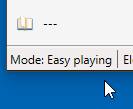
\includegraphics[scale=1.0]{ModeEasyPlaying.png}
		\caption{Easy playing}
		\label{fig:ModeEasyPlaying}
	\end{figure}
	\item \textbf{Playing a game} This is the mode if you play against a chess engine or another player. Only valid chess moves are allowed and the game is time controlled.
	\begin{figure}[H]
		\centering
		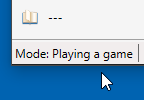
\includegraphics[scale=1.0]{ModePlayingAGame.png}
		\caption{Playing a game}
		\label{fig:ModePlayingAGame}
	\end{figure}
	\item \textbf{Analysing} If you select this mode you can make any chess moves or place the pieces as you like, almost without regard to the chess rules. This mode is recommended to analyse a game or positions. Try different variants on the board and let several chess programs analyse the positions simultaneously. 
	\begin{figure}[H]
		\centering
		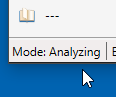
\includegraphics[scale=1.0]{ModeAnalyzing.png}
		\caption{Analysing}
		\label{fig:ModeAnalyzing}
	\end{figure}
	\item \textbf{Analysing a game} If you have loaded a played game and connected to an electronic chessboard, you can analyze the game. Follow the played moves or make some variants and let them be analysed by different chess programs.
    \begin{figure}[H]
	\centering
	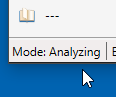
\includegraphics[scale=1.0]{ModeAnalyzing.png}
	\caption{Analysing}
	\label{fig:ModeAnalyzingGame}
\end{figure}
	\item \textbf{Setup Position} Build up a new starting position on the chessboard. It is easiest to set it up on the electronic chessboard.
	\begin{figure}[H]
		\centering
		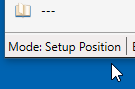
\includegraphics[scale=1.0]{ModeSetupPosition.png}
		\caption{Setup Position}
		\label{fig:ModeSetupPosition}
	\end{figure}
\end{itemize}


\section{Main window}

The first start of BearChess shows the following main window:
\begin{figure}[H]
	\centering
	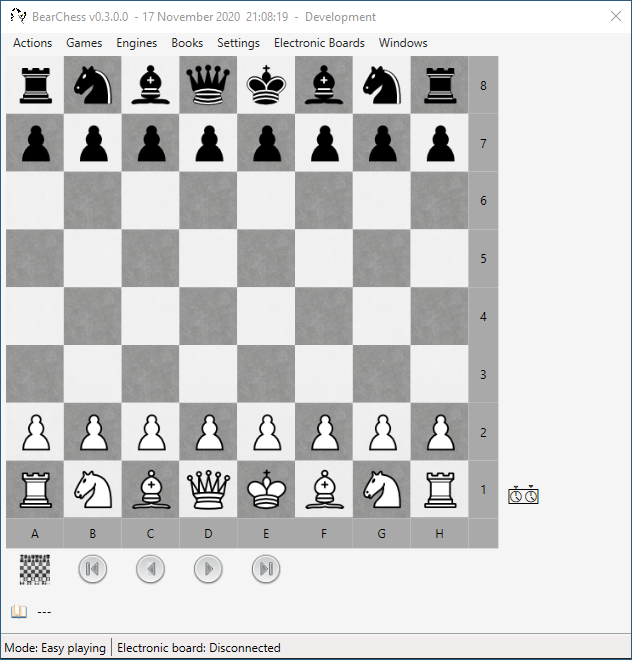
\includegraphics[scale=0.7]{BearChess_MainWindow.png}
	\caption{Main window}
	\label{fig:MainWindow}
\end{figure}

Two buttons are active:
\begin{itemize}
  \item 
\includegraphics[scale=0.5]{arrow_rotate_anticlockwise.png} rotates the board.
  \item 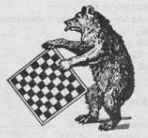
\includegraphics[scale=0.2]{bearchess_2.png} is an easy way to play a game.
Read more in chapter \textbf{\ref{easyStart}  \nameref{easyStart}} on page \pageref{easyStart}.
\end{itemize}
The symbols on the right side give information about the current color and the board rotaion.
\begin{itemize}
	\item 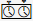
\includegraphics[scale=0.6]{WhiteClock.png} or 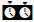
\includegraphics[scale=0.6]{BlackClock.png} for current color.
	\item 
\includegraphics[scale=0.3]{KingW.png}  or 
\includegraphics[scale=0.3]{KingB.png} for board rotation. 
\end{itemize}


\subsection{Actions}
\begin{figure}[H]
	\centering
	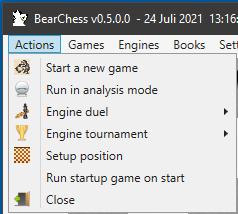
\includegraphics[scale=1.0]{Actions.png}
	\caption{Actions}
	\label{fig:Actions}
\end{figure}
\begin{itemize}
	\item 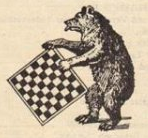
\includegraphics[scale=0.2]{bearchess.png} \textbf{Start a new game} opens a new window to select opponents and time control (see chapter \textbf{\ref{SelectOpponent}  \nameref{SelectOpponent}} on page \pageref{SelectOpponent}).
	
	\item 
\includegraphics[scale=0.5]{robot.png} \textbf{Analysis} allows you to analyze games or positions with suppport of several chess engines (see chapter \textbf{\ref{AnalyzeMode}  \nameref{AnalyzeMode}} on page \pageref{AnalyzeMode})
	
	\item 
\includegraphics[scale=0.5]{6-2-chess-png.png} \textbf{Duel} starts and manage duels (see chapter  \textbf{\ref{EngineDuel}  \nameref{EngineDuel}} on page \pageref{EngineDuel} ).
	
	\item 
\includegraphics[scale=0.5]{cup_gold.png} \textbf{Engine tournament} starts and manage engine tournaments (see chapter  \textbf{\ref{EngineTournamentl}  \nameref{EngineTournamentl}} on page \pageref{EngineTournamentl} ).
	
	\item 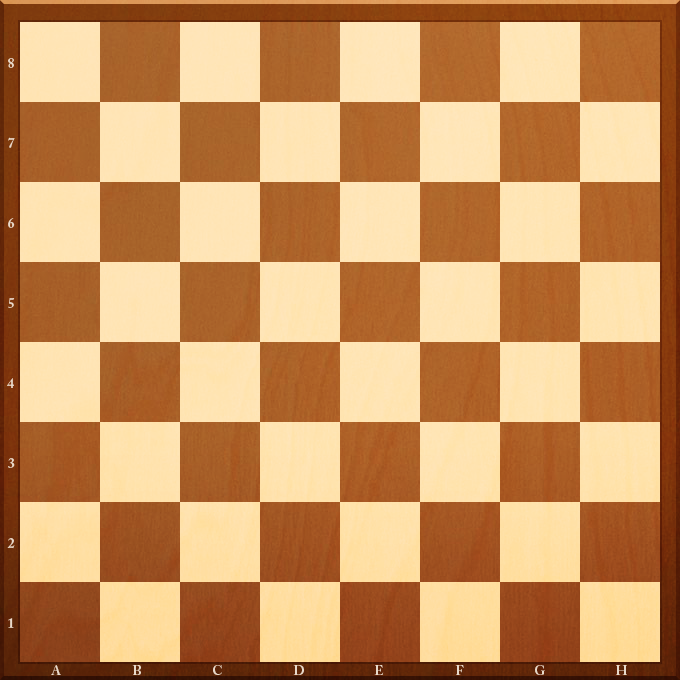
\includegraphics[scale=0.03]{Chess_Board.png} see chapter \textbf{\ref{SetupPosition}  \nameref{SetupPosition}} on page \pageref{SetupPosition}.
	
	\item 
\includegraphics[scale=0.1]{FicsLogo.png} connects you with Free Internet Chess Server (FICS). See chapter \textbf{\ref{FICS}  \nameref{FICS}} on page \pageref{FICS}.	
	
	\item \textbf{Run startup game on start} immediately starts a new game when you start BearChess. For more information read chapter \textbf{\ref{startupgame}  \nameref{startupgame}} on page \pageref{startupgame}.
	
	\item 
\includegraphics[scale=0.5]{door_out.png} \textbf{Close} exits BearChess.
\end{itemize}

\subsection{Games}
\begin{figure}[H]
	\centering
	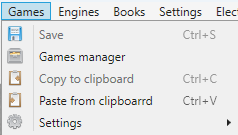
\includegraphics[scale=1.0]{Games1.png}
	\caption{Games}
	\label{fig:Games}
\end{figure}
\begin{itemize}
	\item 
\includegraphics[scale=0.5]{diskette.png} \textbf{Save} your current game.
	\item 
\includegraphics[scale=0.5]{file_manager.png}  \textbf{Games manager} opens a new window in which you can see and load all your previously saved games.
	\item 
\includegraphics[scale=0.5]{clipboard_sign_out.png}  \textbf{Copy to clipboard} copy the current game (PGN) to your clipboard.	
	\item 
\includegraphics[scale=0.5]{clipboard_sign.png}  \textbf{Paste from clipboard} loads a game (PGN) from your clipboard.
	\item 
\includegraphics[scale=0.5]{cog.png}  \textbf{Settings} for show or hide duplicate games.
	
\end{itemize}
All games are saved in a database file. Read more on chapter \textbf{\ref{games}  \nameref{games}} on page \pageref{games}.

\subsection{Engines}
\begin{figure}[H]
	\centering
	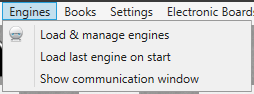
\includegraphics[scale=1.0]{Engines.png}
	\caption{Engines}
	\label{fig:Engines}
\end{figure}
\begin{itemize}
	\item  
\includegraphics[scale=0.5]{robot.png} \textbf{Load \& manage engines} opens a new window in which you can install, load or configure your chess engines.
	\item \textbf{Load last engine on start} if you always want to load immediately an engine when you start BearChess. It has no effect if you have activated the option "Run startup game on start".
	\item \textbf{Show communication window} opens a new window where you can follow the communication between BearChess and chess engines. It is useful to detect any problems in communication.
	\item \textbf{Settings} configure what information you want to see from the engine, e.g. nodes per second.	
\end{itemize}

\subsubsection{Settings}
\begin{figure}[H]
	\centering
	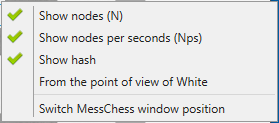
\includegraphics[scale=1.0]{engineSettings.png}
	\caption{Engine Settings}
	\label{fig:EngineSettings}
\end{figure}

\begin{itemize}
	\item  \textbf{Show nodes (N)} How many nodes in the search tree were calculated.
	\item \textbf{Show nodes per seconds (Nps)} How many nodes are calculated per second.
	\item \textbf{Show hash} Utilization of the hash memory in percent.
	\item \textbf{From the point of view of White} Always shows the evaluation value from white's point of view.
	\item \textbf{Switch MessChess window position} If you let \textbf{two} MessChess engines play against each other and the color changes, BearChess will also swap the window position so that the engines for black and white are in the correct order.
\end{itemize}

Read more on chapter \textbf{\ref{loadEngines}  \nameref{loadEngines}} on page \pageref{loadEngines}.

\subsection{Books}
\begin{figure}[H]
	\centering
	\includegraphics[scale=1.0]{Books.png}
	\caption{Books}
	\label{fig:Books}
\end{figure}
\begin{itemize}
	\item 
\includegraphics[scale=0.5]{books_stack.png} \textbf{Load \& manage opening books} opens a new window in which you can install or load  your opening books.
\end{itemize}
BearChess can handle Polyglot and Arena opening books. Read more on chapter \textbf{\ref{OpeningBooks}  \nameref{OpeningBooks}} on page \pageref{OpeningBooks}.

\subsection{Settings}
\begin{figure}[H]
	\centering
	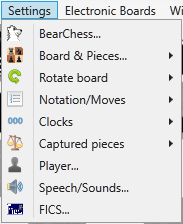
\includegraphics[scale=1.0]{Settings.png}
	\caption{Settings}
	\label{fig:Settings}
\end{figure}
\begin{itemize}
	\item  
\includegraphics[scale=0.9]{Board2DPieces32.png} \textbf{Board \& Pieces} opens a window where you can change the appearance of the chessboard and the pieces.  Read more on chapter \textbf{\ref{BoardAndPieces}  \nameref{BoardAndPieces}} on page \pageref{BoardAndPieces}.
	\item 
\includegraphics[scale=0.5]{arrow_rotate_anticlockwise.png}  \textbf{Rotate board} if the board on the screen should automatically rotate for your color.
	\item  
\includegraphics[scale=0.5]{text_list_numbers.png} \textbf{Notation/Moves} opens a windows where you can change the appearance of the notation, e.g. figurine or letters.
	\item  
\includegraphics[scale=0.5]{digit_separator.png}  \textbf{Clocks} switches between large and small clocks.
	\item  
\includegraphics[scale=0.5]{balance_unbalance.png}  \textbf{Captured pieces} shows the captured pieces window at startup or on demand and you can change the font size to small or big.
	\item  
\includegraphics[scale=0.5]{user_silhouette.png}  \textbf{Player} opens a dialog where you can give it a first and last name.	
    \begin{figure}[H]
	   \centering
    	\includegraphics[scale=1.0]{Player.png}
	    \caption{Player}
 	   \label{fig:Player}
	\end{figure}	
	\item  
\includegraphics[scale=0.5]{sound.png}  \textbf{Sounds} opens a dialog where you can configure some tones that sound when the engine makes a move.
	
    \item 
\includegraphics[scale=0.1]{FicsLogo.png} configure your connection parameters for Free Internet Chess Server (FICS). See chapter \textbf{\ref{FICS}  \nameref{FICS}} on page \pageref{FICS}.		
\end{itemize}

\subsection{Electronic Boards}
\begin{figure}[H]
	\centering
	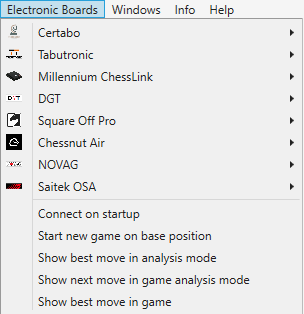
\includegraphics[scale=1.0]{ElectronicBoards.png}
	\caption{Electronic Boards}
	\label{fig:ElectronicBoards}
\end{figure}
\begin{itemize}
	\item  
\includegraphics[scale=0.1]{Certabo_icon.png} \textbf{Certabo} opens a window where you can configure and connect to Certabo chessboards.  Read more on chapter \textbf{\ref{ConfigureCertabo}  \nameref{ConfigureCertabo}} on page \pageref{ConfigureCertabo}.
\item  
\includegraphics[scale=0.05]{tabutronic_logo_def.png} \textbf{TabuTronic} opens a window where you can configure and connect to TabuTronic chessboards (Cerno and Sentio).
Read more on chapter \textbf{\ref{ConfigureTabuTronicCerno}  \nameref{ConfigureTabuTronicCerno}} on page \pageref{ConfigureTabuTronicCerno}.	
or on chapter \textbf{\ref{ConfigureTabuTronicSentio}  \nameref{ConfigureTabuTronicSentio}} on page \pageref{ConfigureTabuTronicSentio}.	
	\item  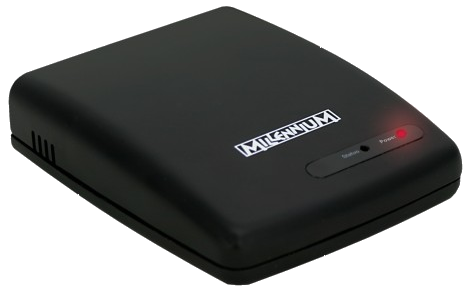
\includegraphics[scale=0.05]{Millennium ChessLink.png} \textbf{Millennium ChessLink} opens a window in which you can configure chessboards connected to Millennium ChessLink and connect to them.  Read more on chapter \textbf{\ref{ConfigureChessLink}  \nameref{ConfigureChessLink}} on page \pageref{ConfigureChessLink}.
	\item  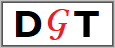
\includegraphics[scale=0.3]{dgt48.png} \textbf{DGT} connect to DGT e-Boards, DGT Revelation or DGT Pegasus chessboard.	
	\item  
\includegraphics[scale=0.05]{squareoff.png} \textbf{Square Off Pro} connect to Square Off Pro chessboard.		
	\item  
\includegraphics[scale=0.1]{chessnut.png} \textbf{Chessnut Air} connect to Chessnut Air chessboard.		
	\item  
\includegraphics[scale=0.3]{novag48.PNG} \textbf{NOVAG} connect to NOVAG Citrine or NOVAG UCB chessboard.			
\item  
\includegraphics[scale=0.4]{Saitek_logo.PNG} \textbf{Saitek OSA} connect to Saitek chessboards with supports OSA protocol.		
	\item \textbf{Connect on startup} tries to connect on to the last connected chessboard when BearChess is started. 	
	\item \textbf{Start a new game on base position} recognizes when you reset all the pieces to the base position during a game. In this case, a new game will be started automatically.
	\item \textbf{Show best move in analysis mode} displays the current best move of the engine on your electronic chessboard.
	\item \textbf{Show best move in game} displays the current best move of the engine on your electronic chessboard.	
\end{itemize}

\subsection{Windows}
\begin{figure}[H]
	\centering
	\includegraphics[scale=1.0]{Windows.png}
	\caption{Windows}
	\label{fig:Windows}
\end{figure}
\begin{itemize}
	\item \textbf{Show} brings clocks or move list windows to the foreground if they are currently not visible.
	\item \textbf{Arrange} auto arange all windows to fit on your screen and not overlapping.
	\item \textbf{Captured pieces} shows the captured pieces. Either all or as a difference. 
\end{itemize}

\subsection{Info}
Opens a window where you can easily go to the path where all configuration is stored.

\subsection{Help}
Opens this document.

\section{Install, Configure and Load a chess engine} \label{loadEngines}

\begin{figure}[H]
	\centering
	\includegraphics[scale=1.0]{LoadEngine.png}
	\caption{Open Load And Manage UCI Engines window}
	\label{fig:LoadEngine}
\end{figure}
BearChess does not include a chess engine. Click on "Load \& manage engines" to install and configure one. "\textit{Install}" means to make a chess program known to BearChess, not to install it on your computer. BearChess supports any UCI engine.\\
\begin{figure}[H]
	\centering
	\includegraphics[scale=1.0]{LoadManageEngine1.png}
	\caption{Load And Manage UCI Engines}
	\label{fig:LoadManageEngine1}
\end{figure}

\begin{itemize}
	\item \includegraphics[scale=0.5]{robot.png} Load selected engine
	\item \includegraphics[scale=0.5]{cog_edit.png} Configure selected engine
	\item \includegraphics[scale=0.5]{file_extension_exe.png} Install a new engine
    \item \includegraphics[scale=0.5]{cog_add.png} Opens a dialog for installing a new engine, which requires parameters to start
	\item \includegraphics[scale=0.5]{bin.png} Uninstall selected engine
	\item \includegraphics[scale=0.5]{door_out.png} Close the window
\end{itemize}

\subsection{Install a new engine} \label{InstallEngine}

To install a new engine click on \includegraphics[scale=0.5]{file_extension_exe.png} and select an UCI engine file, e.g. the Wasp exe file. Or you just drag \& drop the exe file onto the button.\\
If the program needs parameters at the very beginning to be recognized as a UCI chess engine, then click on \includegraphics[scale=0.5]{cog_add.png} and fill out the dialog.\\

\begin{figure}[H]
	\centering
	\includegraphics[scale=1.0]{loadEngine3.png}
	\caption{Load parameter}
	\label{fig:LoadEngine4}
\end{figure}
Aonther way is described in chapter \textbf{\ref{ViaCMDFile}  \nameref{ViaCMDFile}} on page \pageref{ViaCMDFile}.\\

If the file detected as UCI engine, confirm your selection.\\
\begin{figure}[H]
	\centering
	\includegraphics[scale=1.0]{uciConfirm.png}
	\caption{Confirm UCI}
	\label{fig:uciConfirm}
\end{figure}
Next, a configuration dialog box appears where you can configure the engine and give it a name.
\begin{figure}[H]
	\centering
	\includegraphics[scale=0.9]{ConfigureWasp.png}
	\caption{Engine configuration}
	\label{fig:ConfigurWasp}
\end{figure}
The name is freely assignable, must be unique across all engines. But this way you can install the same engine several times with different configurations. The configuration values, names and possibilities are given by the engines. The first time these are the default values.
\begin{itemize}
	\item \includegraphics[scale=0.5]{accept_button.png} Accept the changes
	\item \includegraphics[scale=0.5]{file_extension_log.png} Opens the folder where the log and configration files for this engine are located
	\item \includegraphics[scale=0.5]{undo.png} Reset to default values
	\item \includegraphics[scale=0.5]{cancel.png} Cancel
\end{itemize}
The small \includegraphics[scale=0.3]{folder.png} button, e.g. 'OwnBook\_File', opens a file or directory selection dialog, depending on the configuration name (file, path, dir).\\
The configuration type 'button', e.g. 'Clear Hash', works only if the engine is loaded.

\subsubsection{Wait for a new game} \label{WaitForANewgame}
For the MessChess programs it can be useful not to start immediately but to set parameters first, e.g. an opening book, which are not possible via the UCI configuration.\\
If you enable this option, every time you start a new game with this engine, a dialog will appear waiting for your confirmation.

\begin{figure}[H]
	\centering
	\includegraphics[scale=0.9]{waitNewGame1.png}
	\caption{Wait}
	\label{fig:waitnewGame1}
\end{figure}

If you set a countdown greater than 0 seconds, the confirmation is automatic.

\begin{figure}[H]
\centering
\includegraphics[scale=0.9]{waitNewGame2.png}
\caption{Countdown}
\label{fig:waitnewGame2}
\end{figure}




\subsubsection{Assign a logo file}
The small \includegraphics[scale=0.3]{folder.png} button on the 'Logo:' line opens a file selection dialog where you can choose a logo file for this engine.

\begin{figure}[H]
	\centering
	\includegraphics[scale=0.9]{logoFile.png}
	\caption{Engine Logo file}
	\label{fig:LogoFile}
\end{figure}

\subsubsection{Add start parameter}
You can enter a start parameter if the engine needs one.
\begin{figure}[H]
	\centering
	\includegraphics[scale=0.9]{engineParameter.png}
	\caption{Engine Paramater}
	\label{fig:EngineParameter}
\end{figure}

\subsubsection{Use opening book}
Some engines come with their own opening book and you have an option to use them or not. You can also tell BearChess to use an opening book before the moves are calculated by the engines. You can configure how BearChess determines the book move. 
\begin{itemize}
	\item \textbf{Best} Always chooses the best move
	\item \textbf{Flexible} Selects one of the best moves
    \item \textbf{Wide} Selects any book move
\end{itemize}
Look at chapter \textbf{\ref{OpeningBooks}  \nameref{OpeningBooks}} on page \pageref{OpeningBooks} how to install an opening book.

\subsubsection{Install Certabo Avatar UCI Chess engine}
Certabo provides a special engine, called Avatar UCI Chess engine (look at \url{https://www.avataruci.org/}).\\
This engine is not intended for super strong players but tries to replicate your style. It learns from your games (you do not need many many thousand), it can start with some tens or hundreds. Certabo has a learning algohrithm which creates some weights and opening books emulating personality. Certabo created avatars of some players from the past and you can find them in the latest Certabo software. Just select Avatar as main engine and you will be prompted to choose the Avatar you want to play.\\
You can use this engine in BearChess too. 
If you have installed the latest Certabo software (Version 4.5 or above), select the avatar.exe file from the engines subfolder as the new engine. BearChess looks at the 'avatar\_weights' subfolder and asks you to select an avatar.

\begin{figure}[H]
	\centering
	\includegraphics[scale=0.9]{avatar1.png}
	\caption{Select an avatar}
	\label{fig:Avatar1}
\end{figure}

\begin{figure}[H]
	\centering
	\includegraphics[scale=0.9]{avatar2.png}
	\caption{Confirm}
	\label{fig:Avatar2}
\end{figure}

\begin{figure}[H]
	\centering
	\includegraphics[scale=0.7]{avatar3.png}
	\caption{Configure}
	\label{fig:Avatar3}
\end{figure}

There are no other configuration options. In the bottom line you can see the required parameters for the avatar engine.\\
If you don't find the right avatar, click on the small folder icon and you can select another avatar file, e.g. your personally created file from Certabo.

\begin{figure}[H]
	\centering
	\includegraphics[scale=0.7]{avatar4.png}
	\caption{Select your avatar}
	\label{fig:Avatar4}
\end{figure}

\subsubsection{Install MessChess engine}
Franz Huber provides emulator software to play against old chess computers as UCI engine (look at \url{https://fhub.jimdofree.com/}).\\
If you have downloaded und unzipped the latest version of CB-Emu, select the MessChess.exe file from the MessChess subfolder as the new engine. BearChess reads the Engines.lst file and ask you to select one or more chess computer emulations.

\begin{figure}[H]
	\centering
	\includegraphics[scale=0.8]{MessChess1.png}
	\caption{Select an emulation}
	\label{fig:MessChess1}
\end{figure}

You can select more than one engine to facilitate the installation of multiple emulations in one step. The filter input field allows you to reduce the list.

\begin{figure}[H]
	\centering
	\includegraphics[scale=0.8]{MessChess5.png}
	\caption{Filter the list}
	\label{fig:MessChess5}
\end{figure}

If you check the option "Skip error....", BearChess will not show an error if you try to install an already installed emulation.

\begin{figure}[H]
	\centering
	\includegraphics[scale=0.9]{MessChess2.png}
	\caption{Confirm}
	\label{fig:MessChess2}
\end{figure}

There are only some configuration options. In the bottom line you can see the required parameters for the engine.

\begin{figure}[H]
	\centering
	\includegraphics[scale=0.8]{MessChess3.png}
	\caption{Configure}
	\label{fig:MessChess3}
\end{figure}

If you need to set some more options, see \textbf{\ref{WaitForANewgame}  \nameref{WaitForANewgame}} on page \pageref{WaitForANewgame}.

\subsubsection{Install an engine via CMD file} \label{ViaCMDFile}
If an engine needs special parameters or a parameter to be recognized as a UCI engine, you can use a CMD file instead of the EXE file. Write all required commands into the CMD file and install.

\begin{figure}[H]
	\centering
	\includegraphics[scale=0.8]{LoadEngineCmd.png}
	\caption{Load CMD file}
	\label{fig:LoadCMDfile}
\end{figure}


\subsection{Configure an engine}

To change the configuration of an installed engine click on \includegraphics[scale=0.5]{cog.png}\\
The same configuration dialog box as during installation is shown where you can configure the engine or just change the name.

\subsection{Additional configuration for an installed engine}

If you want to save the same engine with a different configuration, e.g. an additional configuration with adjusted Elo strength, you can save the configuration under a different name.

\begin{figure}[H]
	\centering
	\includegraphics[scale=0.8]{ConfigureWasp_2.png}
	\caption{Save as new configuration}
	\label{fig:LoadEngine3}
\end{figure}
Click on \includegraphics[scale=0.5]{cog_add.png} to save the configuration with a new name.\\


\subsection{Load an engine}

To load an installed engine, select an engine and click on \includegraphics[scale=0.5]{robot.png} or just double-click.

\begin{figure}[H]
	\centering
	\includegraphics[scale=1.0]{LoadEngine2.png}
	\caption{Some installed engines}
	\label{fig:LoadEngine2}
\end{figure}


\subsubsection{Load a MessChess engine}

When you load a MessChess engine the emulation window will appear too.
\begin{figure}[H]
	\centering
	\includegraphics[scale=0.7]{MessChess4.png}
	\caption{Academy}
	\label{fig:MessChess4}
\end{figure}
Use only BearChess or your electronic chessboard to make any moves. You can use the emulaton window to set options, e.g. levels or time control.\\
{\color{red}\textbf{*}} When you play a game against a MessChess engine, the selected time control for the game cannot be transferred to the emulation. To avoid, that BearChess ends the game too early by timeout, you should select here only an average time per move.

\subsubsection{Load an engine by command line}
If you like to load an engine at startup, you can add a command line parameter \textbf{-engine} folllowed by the engine name:
\begin{verbatim}
 BearChessWin.exe -engine "Stockfish 12"
\end{verbatim}
{\color{red}\textbf{*}} The engine name must match the name in the list of installed engines.

\section{Load and Manage Opening Books} \label{OpeningBooks}

\begin{figure}[H]
	\centering
	\includegraphics[scale=1.0]{books.png}
	\caption{Open Load and Manage Opening Books  }
	\label{fig:LoadManageBooks1}
\end{figure}

BearChess does not include opening books. Click on "Load \& manage opening books" to install one. "\textit{Install}" means to make a opening book known BearChess, not to install it on your computer. BearChess supports Polyglot and Arena opening books.\\

\begin{figure}[H]
	\centering
	\includegraphics[scale=1.0]{LoadManageBooks2.png}
	\caption{Load and Manage Opening Books  }
	\label{fig:LoadManageBooks2}
\end{figure}

\begin{itemize}
	\item \includegraphics[scale=0.5]{book_open.png} Load selected book
	\item \includegraphics[scale=0.5]{book_add.png} Install a new book
	\item \includegraphics[scale=0.5]{bin.png} Uninstall selected book
	\item \includegraphics[scale=0.5]{door_out.png} Close the window
\end{itemize}

To install a new opening book, click on \includegraphics[scale=0.5]{book_add.png} and select a book file. The file extension for Polyglot books is \textbf{bin} and for Arena is \textbf{abk}.

\begin{figure}[H]
	\centering
	\includegraphics[scale=1.0]{LoadManageBooks3.png}
	\caption{Some installed books }
	\label{fig:LoadManageBooks3}
\end{figure}

To select an opening book, click on \includegraphics[scale=0.5]{book_open.png} or just double-click. 
A new window opens and shows the current possible moves found in the book.

\begin{figure}[H]
	\centering
	\includegraphics[scale=1.0]{OpeningBook.png}
	\caption{Loaded opening book on base position }
	\label{fig:OpeningBook}
\end{figure}

You can load more than one book. Every book has its own window and is synchronized with the current position on the chessboard.

\begin{figure}[H]
	\centering
	\includegraphics[scale=0.8]{OpeningBook2.png}
	\caption{Loaded opening books }
	\label{fig:OpeningBook2}
\end{figure}

{\color{red}\textbf{*}} So far, the possibilities are still very limited with the opening books. This will improve in the next versions. 

\section{Configure Board and Pieces} \label{BoardAndPieces}

\begin{figure}[H]
	\centering
	\includegraphics[scale=1.0]{SettingsBoardAndPieces.png}
	\caption{Open window to configure board and pieces }
	\label{fig:SettingsBoardAndPieces}
\end{figure}

To change the appearance of BearChess select "Board and Pieces". A new window opens where you can configure it. 

\begin{figure}[H]
	\centering
	\includegraphics[scale=0.9]{SettingsBoardAndPieces2.png}
	\caption{Setup board and pieces }
	\label{fig:SettingsBoardAndPieces2}
\end{figure}

BearChess comes with several set of pieces and board colors. \textbf{Many thanks to Bryan Whitby and Certabo for permission to use their design.}

\begin{figure}[H]
	\centering
	\includegraphics[scale=0.9]{SettingsBoardAndPieces3.png}
	\caption{Pre-installed pieces }
	\label{fig:SettingsBoardAndPieces3}
\end{figure}

\begin{figure}[H]
	\centering
	\includegraphics[scale=0.9]{SettingsBoardAndPieces4.png}
	\caption{Pre-installed boards}
	\label{fig:SettingsBoardAndPieces4}
\end{figure}


\begin{itemize}
	\item \includegraphics[scale=0.5]{file_manager.png} Install new board colors or pieces
	\item \includegraphics[scale=0.5]{bin.png} Uninstall board colors or pieces
	\item \includegraphics[scale=0.5]{accept_button.png} Accept the changes
	\item \includegraphics[scale=0.5]{cancel.png} Cancel
\end{itemize}




\subsection{Install new board colors and pieces}
BearChess uses png files for board colors and pieces.

\subsubsection{New board colors}
Click on \includegraphics[scale=0.5]{file_manager.png} to select a directory where the files are located. BearChess accepts \verb|w.png| or \verb|white.png| for white fields and \verb|b.png| or \verb|black.png| for black fields.

\begin{figure}[H]
	\centering
	\includegraphics[scale=1.0]{WoodPieces.png}
	\caption{Example for wood fields }
	\label{fig:WoodPieces}
\end{figure}

If BearChess finds both files inside the directory, it builds an empty chessboard to confirm your choice. A name for your board is required.

\begin{figure}[H]
	\centering
	\includegraphics[scale=1.0]{ConfirmBoard.png}
	\caption{Confirm new board }
	\label{fig:ConfirmBoard}
\end{figure}

\subsubsection{New pieces}
There are two ways to install a new set of pieces. One png file for each piece or one png file with all pieces inside. \\
Click on \includegraphics[scale=0.5]{file_manager.png} to select a directory where the files are located.\\ \textbf{Important:} The png files must have a transparent background color, otherwise they would paint over the fields.
BearChess accepts following names for the different pieces:
\begin{itemize}
	\item \textbf{White king:} \verb|KingW.png, WhiteKing.png, wk.png|
	\item \textbf{Black king:} \verb|KingB.png, BlackKing.png, bk.png|
	\item \textbf{White queen:} \verb|QueenW.png, WhiteQueen.png, wq.png|
	\item \textbf{Black queen:} \verb|QueenB.png, BlackQueen.png, bq.png|
	\item \textbf{White rook:} \verb|RookW.png, WhiteRook.png, wr.png|
	\item \textbf{Black rook:} \verb|RookB.png, BlackRook.png, br.png|
	\item \textbf{White bishop:} \verb|BishopW.png, WhiteBishop.png, wb.png|
	\item \textbf{Black bishop:} \verb|BishopB.png, BlackBishop.png, bb.png|
	\item \textbf{White knight:} \verb|KnightW.png, WhiteKnight.png, wn.png|
	\item \textbf{Black knight:} \verb|KnightB.png, BlackKnight.png, bn.png|
	\item \textbf{White pawn:} \verb|PawnW.png, WhitePawn.png, wp.png|
	\item \textbf{Black pawn:} \verb|PawnB.png, BlackPawn.png, bp.png|
\end{itemize}


\begin{figure}[H]
	\centering
	\includegraphics[scale=0.7]{Pieces.png}
	\caption{Example one png file for each piece}
	\label{fig:Pieces}
\end{figure}

If BearChess finds all files inside the directory, it builds a piece set to confirm your choice.\\

If BearChess finds only one png file inside the directory, it assumes that this file contains all pieces at once.

\begin{figure}[H]
	\centering
	\includegraphics[scale=6.5]{Leipzig.png}
	\caption{One png file with all pieces}
	\label{fig:Leipzig}
\end{figure}

The png must have the pieces in the order and colors shown above.\\
If you have one png file for all pieces, you can just drag \& drop the png file onto the
open file dialog icon. It avoids the effort to have a separate directory for each file.
\begin{figure}[H]
	\centering
	\includegraphics[scale=0.9]{DropPieceSet.png}
	\caption{Drop new pieces }
	\label{fig:DropPieceSet}
\end{figure}

\begin{figure}[H]
	\centering
	\includegraphics[scale=0.9]{ConfirmPieces.png}
	\caption{Confirm new pieces }
	\label{fig:ConfirmPieces}
\end{figure}

BearChess builds a piece set to confirm your choice. A name for your set is required.
Now you can combine your boards with your pieces.

\begin{figure}[H]
	\centering
	\includegraphics[scale=0.8]{CombineBoardPieces.png}
	\caption{Combine board and pieces }
	\label{fig:CombineBoardPieces}
\end{figure}

\subsection{Show last/best move}
If the options "Show last move" and "Show best move" are activated, the last move and the currently best analysis move of an engine are marked on the board.


\begin{figure}[H]
	\centering
	\includegraphics[scale=0.8]{LastMoveArrow.png}
	\caption{Last/best move as arrow}
	\label{fig:LastMove2}
\end{figure}

\subsection{Possible moves}
If the option "Show possible moves" activated, all possible moves are indicated by an arrow.
Either when the mouse pointer hovers over a target field or over a piece.


\begin{figure}[H]
	\centering
	\includegraphics[scale=0.8]{SettingsBoardAndPieces5.png}
	\caption{Show possible moves for target field}
	\label{fig:ShowPossibleMoves}
\end{figure}


\begin{figure}[H]
	\centering
	\includegraphics[scale=0.8]{SettingsBoardAndPieces6.png}
	\caption{Show possible moves for pieces}
	\label{fig:ShowPossibleMoves2}
\end{figure}

You can define the arrow color.


\section{Configure Notation and Moves}
\begin{figure}[H]
	\centering
	\includegraphics[scale=0.9]{NotationAndMoves1.png}
	\caption{Opens a window to configure notation and moves }
	\label{fig:NotationAndMoves}
\end{figure}
BearChess can display moves in different ways.
\begin{figure}[H]
	\centering
	\includegraphics[scale=1.0]{NotationAndMoves2.png}
	\caption{Configure notation and moves }
	\label{fig:NotationAndMoves2}
\end{figure}
In long and short notation and with symbols or letters for the chessmen.
You can change the language for the letters by clicking on the country flag.
This has an effect on the move list and the output on the DGT chess clocks and Revelation respectively.

\section{Configure clock style}
\begin{figure}[H]
	\centering
	\includegraphics[scale=1.0]{ConfigureClocks.png}
	\caption{Configure clocks }
	\label{fig:ConfigureClocks}
\end{figure}

BearChess offers two different clocks: small and big

\begin{figure}[H]
	\centering
	\includegraphics[scale=1.0]{SmallClocks.png}
	\caption{Small clocks }
	\label{fig:SmallClocks}
\end{figure}
\begin{figure}[H]
	\centering
	\includegraphics[scale=0.8]{BigClocks.png}
	\caption{Big clocks }
	\label{fig:BigClocks}
\end{figure}

\section{Configure speech and sounds}

\begin{figure}[H]
	\centering
	\includegraphics[scale=1.0]{Sounds2.png}
	\caption{Sounds }
	\label{fig:Sounds2}
\end{figure}
Opens a window where you can configure some sounds.

\begin{figure}[H]
	\centering
	\includegraphics[scale=1.0]{Sounds1.png}
	\caption{Speech and sound configuration}
	\label{fig:Sounds1}
\end{figure}	

Here you can set whether BearChess should announce moves or other events in your language or only play a sound when the engine makes a move, gives check or mates. Optionally you can also configure an individual sound file. Only wave files are supported. Only either voice output or playing sounds can be enabled.

\subsection{Configure speech}

\begin{itemize}
  \item The "\textbf{Speech active}" checkbox activates speech output.
  \item You can choose between two types of move announcements: The long version, e.g. "Knight from g1 to f3" or the short version "Knight f3".
  \item If you activate the "Own move" checkbox, your moves will also be announced. This can be usefull for boards without LEDs to verify that the move is recognized by BearChess.
  \item The "\textbf{Language}" table shows all the languages installed for the speech output. BearChess does not deliver any language files itself. Choose your preferred language. 
\end{itemize}
If you choose English or German, BearChess knows all required words for full support of both languages.\\
If not or you want to change some words or you want BearChess to greet you individually, activate "Define your own translation" and click the button \includegraphics[scale=0.5]{world_edit.png}.

 \begin{figure}[H]
	\centering
	\includegraphics[scale=0.7]{Sounds3.png}
	\caption{Define translation}
	\label{fig:Sounds3}
\end{figure}
Just type the words in your language into the fields. For example, if you want to hear "mate" instead of "check mate", enter it in the field next to "check mate:".\\
Or if your are Italian, enter all fields with your language, for example "re" for king and "donna" for queen.\\
{\color{red}*} The speech output is asynchronous and does not slow down the game. However, all texts are always spoken. If there is a fast sequence of moves, the output may lag behind the game.

\subsection{Configure sound}

When the speech output is not active, you can activate some sound effects and also select your own wave files.

\begin{itemize}
	\item \includegraphics[scale=0.5]{sound.png} Play the sound
	\item \includegraphics[scale=0.5]{file_extension_wav.png} Opens a files selection dialog for an individual sound file.
	\item \includegraphics[scale=0.5]{delete.png} Removes the sound file selection.
\end{itemize}


\section{Show captured pieces}
\begin{figure}[H]
	\centering
	\includegraphics[scale=1.0]{CapturedPieces1.png}
	\caption{Show captured pieces }
	\label{fig:CapturedPieces1}
\end{figure}

Opens a window that shows the captured pieces.
\begin{figure}[H]
	\centering
	\includegraphics[scale=1.0]{CapturedPieces2.png}
	\caption{Show captured pieces on start }
	\label{fig:CapturedPieces2}
\end{figure}
You can configure this window so that it is displayed at startup.

\begin{figure}[H]
	\centering
	\includegraphics[scale=1.0]{CapturedPieces3.png}
	\caption{Show all captured pieces }
	\label{fig:CapturedPieces3}
\end{figure}

Figure \ref{fig:CapturedPieces3} shows all captured pieces.

\begin{figure}[H]
	\centering
	\includegraphics[scale=1.0]{CapturedPieces4.png}
	\caption{Show captured pieces as difference}
	\label{fig:CapturedPieces4}
\end{figure}
Figure \ref{fig:CapturedPieces4} shows the same information as difference.

The button \includegraphics[scale=0.5]{balance_unbalance.png} switches between both views.


\section{Electronic chessboards} \label{ElectronicChessBoard}
BearChess supports many electronic chessboards: \textbf{Certabo} and \textbf{TabuTronic}  boards, \textbf{Millennium} boards via the ChessLink module (incl. \textbf{eOne}), \textbf{DGT e-Boards} (incl. Revelation), \textbf{DGT Pegasus}, \textbf{Square Off Pro}, \textbf{Chessnut Air}, \textbf{NOVAG} and \textbf{Saitek} boards. Certabo, TabuTronic, Millennium boards and DGT e-Boards communicate via an USB port as serial COM port or via Bluetooth. DGT Pegasus and Square Off Pro communicate only via Bluetooth. Which COM port is used is not the same for all computers and can change over time, especially if you have more than one COM port available on your computer. Chessnut Air communicates via an USB port as a Human Interface Device (HID) or via Bluetooth LE.\\ 
For Bluetooth, BearChess distinguishes between the classic (no official designation, but used here) and the Low Energy (LE) variant.
In the classic variant, pairing is necessary and the connection is then made to a serial COM port. The LE variant is even more user-friendly. No pairing is necessary and there is no conversion to a COM port.

\subsection{Configure Certabo boards} \label{ConfigureCertabo}
\begin{figure}[H]
	\centering
	\includegraphics[scale=1.0]{Certabo1.png}
	\caption{Open a window to configure Certabo boards }
	\label{fig:Certabo1}
\end{figure}

Certabo requires two configuration steps. The used COM port and a calibration to detect the chess pieces. If your PC supports bluetooth and you own the Bluetooth module from Certabo, you can also connect to the Certabo board via bluetooth. If you want to do this, check the option "Bluetooth" first, before opening the configuration window.\\
The piece recognition assumes that the USB port of the board is on the bottom right.

\begin{figure}[H]
	\centering
	\includegraphics[scale=1.0]{Certabo6.png}
	\caption{Search for Bluetooth }
	\label{fig:Certabo6}
\end{figure}

Read chapter \textbf{\ref{CertaboBluetooth}  \nameref{CertaboBluetooth}} on page \pageref{CertaboBluetooth} for more information.

\begin{figure}[H]
	\centering
	\includegraphics[scale=1.0]{Certabo2.png}
	\caption{Configure Certabo boards }
	\label{fig:Certabo2}
\end{figure}

Select the COM port (BT for Bluetooth) if you know it or use the <auto> selection. 
Click on \includegraphics[scale=0.5]{connect.png} to verify your selection.

\begin{figure}[H]
	\centering
	\includegraphics[scale=0.9]{Calibrate1.png}
	\caption{COM port successful detected}
	\label{fig:Calibrate1}
\end{figure}

If you select an invalid COM port, you will see the following error message:

\begin{figure}[H]
	\centering
	\includegraphics[scale=0.9]{Calibrate2.png}
	\caption{Invalid COM port }
	\label{fig:Calibrate2}
\end{figure}

If you select <auto> and no board is found, you will receive the following error message:

\begin{figure}[H]
	\centering
	\includegraphics[scale=0.9]{Calibrate3.png}
	\caption{No board found }
	\label{fig:Calibrate3}
\end{figure}

\textbf{Hint:} You can always use the selection <auto>, but if you have more than one COM port available, it can take some seconds until the right one is recognized.

\subsubsection{Configure Bluetooth} \label{CertaboBluetooth}

If the "Bluetooth" option is set, the following window will be displayed for a short time if you open the configuration dialog.

\begin{figure}[H]
	\centering
	\includegraphics[scale=0.8]{MillenniumChessLink10.png}
	\caption{Search for Bluetooth}
	\label{fig:CertaboBT10}
\end{figure}

During this time or if you connect for the first time, Windows may ask you to connect to the module. In this case, confirm this. 

\subsubsection{Calibration}
At the first start, BearChess needs a calibration to identify your chessmen. A new calibration is only required if you use another set of chessmen.\\
Click on \includegraphics[scale=0.08]{chessboard_base.png} to open the calibration dialog.
\begin{figure}[H]
	\centering
	\includegraphics[scale=1.0]{CalibrateBase.png}
	\caption{Calibrate base position }
	\label{fig:CalibrateBase}
\end{figure}
If all pieces on the correct position, click the \includegraphics[scale=0.5]{accept_button.png} button. When a calibration is running, you will see the chessboard LEDs flashing. Please wait until all LEDs are off and the confirm dialog appears.

\begin{figure}[H]
	\centering
	\includegraphics[scale=1.0]{Calibrate4.png}
	\caption{Calibration finished }
	\label{fig:Calibrate4}
\end{figure}

\textbf{Hint:} If the calibration never seems to end, check that the chessmen are correctly placed in the middle of the squares.

\subsubsection{Connect}
\begin{figure}[H]
	\centering
	\includegraphics[scale=1.0]{Certabo3.png}
	\caption{Connect to Certabo}
	\label{fig:Certabo3}
\end{figure}
When the configuration is complete, you can connect your chessboard.
In the lower right corner appears a new button, which allows you to easily connect or disconnect your board. The current status is also displayed.

\begin{figure}[H]
	\centering
	\includegraphics[scale=0.8]{Certabo4.png}
	\caption{Connected}
	\label{fig:Certabo4}
\end{figure}

\begin{figure}[H]
	\centering
	\includegraphics[scale=0.8]{Certabo5.png}
	\caption{Disconnected}
	\label{fig:Certabo5}
\end{figure}

\subsection{Configure TabuTronic Cerno} \label{ConfigureTabuTronicCerno}

\begin{figure}[H]
	\centering
	\includegraphics[scale=0.8]{Cerno1.png}
	\caption{Open a window to configure TabuTronic Cerno}
	\label{fig:Cerno1}
\end{figure}

The configuration is exactly as it is for the Certabo boards.
Read more on chapter \textbf{\ref{ConfigureCertabo}  \nameref{ConfigureCertabo}} on page \pageref{ConfigureCertabo}.

\subsection{Configure TabuTronic Sentio} \label{ConfigureTabuTronicSentio}

\begin{figure}[H]
	\centering
	\includegraphics[scale=0.8]{Sentio1.png}
	\caption{Open a window to configure TabuTronic Sentio }
	\label{fig:Sentio1}
\end{figure}


\begin{figure}[H]
	\centering
	\includegraphics[scale=1.0]{Sentio2.png}
	\caption{Select COM port}
	\label{fig:Sentio2}
\end{figure}

Select the COM port if you know it or use the <auto> selection. 
Click on \includegraphics[scale=0.5]{connect.png} to verify your selection.

\subsubsection{Configure Bluetooth} \label{SentioBluetooth}

If the "Bluetooth" option is set, the following window will be displayed for a short time if you open the configuration dialog.

\begin{figure}[H]
	\centering
	\includegraphics[scale=0.8]{MillenniumChessLink10.png}
	\caption{Search for Bluetooth}
	\label{fig:SentioBT10}
\end{figure}

During this time or if you connect for the first time, Windows may ask you to connect to the module. In this case, confirm this.

\subsubsection{Connect}
\begin{figure}[H]
	\centering
	\includegraphics[scale=0.8]{Sentio3.png}
	\caption{Connect to TabuTronic Sentio}
	\label{fig:Sentio3}
\end{figure}
When the configuration is complete, you can connect your chessboard.
In the lower right corner appears a new button, which allows you to easily connect or disconnect your board. The current status is also displayed.
\\TabuTronic Sentio has no real piece recognition and can only give the information per field whether there is a piece or not.


\subsection{Configure Millennium ChessLink} \label{ConfigureChessLink}
\begin{figure}[H]
	\centering
	\includegraphics[scale=1.0]{MillenniumChessLink1.png}
	\caption{Open a window to configure Millennium boards }
	\label{fig:MillenniumChessLink1}
\end{figure}

For your Millennium ChessLink you may need to configure if you want to use a COM port or Bluetooth. You can also change how the LEDs should light up.\\
If your PC supports Bluetooth, you can also connect to the ChessLink module via Bluetooth. If you want to do this, check the option "Bluetooth Classic" and/or "Bluetooth LE" first, before opening the configuration windows.\\
The piece recognition assumes that the cable is on the right side of the board.

\begin{figure}[H]
	\centering
	\includegraphics[scale=0.8]{MillenniumChessLink9.png}
	\caption{Search for Bluetooth }
	\label{fig:MillenniumChessLink9}
\end{figure}
Read chapter \textbf{\ref{Bluetooth}  \nameref{Bluetooth}} on page \pageref{Bluetooth} for more information.

\begin{figure}[H]
	\centering
	\includegraphics[scale=0.9]{MillenniumChessLink2.png}
	\caption{Configure Millennium ChessLink}
	\label{fig:MillenniumChessLink2}
\end{figure}

Select the COM port if you know it or use the <auto> selection.
Click on \includegraphics[scale=0.5]{connect.png} to verify your selection.

\begin{figure}[H]
	\centering
	\includegraphics[scale=1.0]{MillenniumChessLink3.png}
	\caption{COM port successful detected }
	\label{fig:MillenniumChessLink3}
\end{figure}

If you select an invalid COM port,e.G. COM7, you will see the following error message:

\begin{figure}[H]
	\centering
	\includegraphics[scale=1.0]{MillenniumChessLink4.png}
	\caption{Invalid COM port }
	\label{fig:MillenniumChessLink4}
\end{figure}

If you select <auto> and no board is found, you will receive the following error message:

\begin{figure}[H]
	\centering
	\includegraphics[scale=1.0]{MillenniumChessLink5.png}
	\caption{No board found }
	\label{fig:MillenniumChessLink5}
\end{figure}

\textbf{Hint:} You can always use the selection <auto>, but if you have more than one COM port available, it can take some seconds until the right one is recognized.\\

\subsubsection{LEDs}
You can change the brightness of the LEDs and whether they should or synchronously when indicating moves.\\
Use the slider to change the brightness from dim to light.\\
A click on \includegraphics[scale=0.4]{eye.png} connects to the board and you can see the changes live.

\subsubsection{Delay}
You can define a delay how fast the board, after detecting a change, reports this to BearChess. A delay supports the possibility to move pieces slower across the board before BearChess recognizes the change as a move. \\
\begin{figure}[H]
	\centering
	\includegraphics[scale=1.0]{MillenniumChessLink11.png}
	\caption{Delay}
	\label{fig:MillenniumChessLink11}
\end{figure}
Valid values ranges from 0 (no delay) to 4. Default value is 0.


\subsubsection{Scans}
You can specify how often internally within a second the board is checked for changes.\\
\begin{figure}[H]
	\centering
	\includegraphics[scale=1.0]{MillenniumChessLink12.png}
	\caption{Scan}
	\label{fig:MillenniumChessLink12}
\end{figure}
Valid values ranges from 32.6 to 1.9 per second. Default ist 16.3 per second.
Changing the scan rate allows a finer adjustment of how fast a board change is reported to BearChess. But the influence is less than the delay setting.

\subsubsection{Configure Bluetooth} \label{Bluetooth}

If the "Bluetooth Classic" option is set, the following window will be displayed for a short time if you open the configuration dialog.

\begin{figure}[H]
	\centering
	\includegraphics[scale=0.8]{MillenniumChessLink10.png}
	\caption{Search for Bluetooth}
	\label{fig:MillenniumChessLink10}
\end{figure}

During this time or if you connect for the first time, Windows may ask you to connect to the Millennium ChessLink module. In this case, confirm this.\\

If the "Bluetooth LE" option is set, the connection is not emulated as a serial COM port. The configuration shows the port name as "BTLE".


\subsubsection{Connect}
\begin{figure}[H]
	\centering
	\includegraphics[scale=1.0]{MillenniumChessLink6.png}
	\caption{Connect to Millennium ChessLink}
	\label{fig:MillenniumChessLink6}
\end{figure}
When the configuration is complete, you can connect to your chessboard.
In the lower right corner appears a new button, which allows you to easily connect or disconnect your board. The current status is also displayed.

\begin{figure}[H]
	\centering
	\includegraphics[scale=0.8]{MillenniumChessLink7.png}
	\caption{Connected}
	\label{fig:MillenniumChessLink7}
\end{figure}

\begin{figure}[H]
	\centering
	\includegraphics[scale=0.8]{MillenniumChessLink8.png}
	\caption{Disconnected}
	\label{fig:MillenniumChessLink8}
\end{figure}

\subsection{Configure DGT e-Board} \label{ConfigureDGTEBoard}
\begin{figure}[H]
	\centering
	\includegraphics[scale=0.8]{DGTEBoard1.png}
	\caption{Open a window to configure DGT e-boards }
	\label{fig:DGTEBoard1}
\end{figure}

For your DGT e-Board or Revelation you may need to configure if you want to use a COM port or Bluetooth. 
If your PC \textbf{and} your e-Board supports Bluetooth, you can also connect to the e-Board via Bluetooth. If you want to do this, check the option "Bluetooth" first, before opening the configuration windows.\\
Read chapter \textbf{\ref{BluetoothDGT}  \nameref{BluetoothDGT}} on page \pageref{BluetoothDGT} for more information.

\begin{figure}[H]
	\centering
	\includegraphics[scale=1.0]{DGTEBoard2.png}
	\caption{Configure DGT e-boards }
	\label{fig:DGTEBoard2}
\end{figure}

You can use an external clock (DGT3000, DGTPi) or the Revelation display to display moves and time.
\begin{itemize}
	\item Activate "\textbf{Clock}" if you use a clock.
	\item Activate the "Change side" checkbox if your clock is set on the right side. Normally, the clock is set to the left side for a white player. 
	\item Activate "Show only moves" if you do not want to display your time on the clock.
	\item Select how you want the moves to be displayed on the clock.
\end{itemize}


\subsubsection{Configure Bluetooth} \label{BluetoothDGT}

If the "Bluetooth" option is set, the following window will be displayed for a short time if you open the configuration dialog.

\begin{figure}[H]
	\centering
	\includegraphics[scale=0.8]{MillenniumChessLink10.png}
	\caption{Search for Bluetooth}
	\label{fig:DGTEBoardBT}
\end{figure}

During this time or if you connect for the first time, Windows may ask you to connect to the DGT e-Board and maybe you have to enter a pairing code. For more details, read the e-Board user manual.\\


\subsection{Connect DGT Pegasus} \label{ConfigurePegasus}
\begin{figure}[H]
	\centering
	\includegraphics[scale=0.8]{Pegasus1.png}
	\caption{Connect to DGT Pegasus }
	\label{fig:Pegasus1}
\end{figure}

No configuration is required for your DGT Pegasus chessboard.\\
DGT Pegasus requires a Bluetooth LE connection. Make sure that your Bluetooth adapter also supports LE.

\begin{figure}[H]
	\centering
	\includegraphics[scale=0.8]{Pegasus2.png}
	\caption{Connected}
	\label{fig:Pegasus2}
\end{figure}

\begin{figure}[H]
	\centering
	\includegraphics[scale=0.8]{Pegasus3.png}
	\caption{Disconnected}
	\label{fig:Pegasus3}
\end{figure}

After a successful connection, you need to confirm that the pieces are all in the correct position.

\begin{figure}[H]
	\centering
	\includegraphics[scale=0.8]{Pegasus4.png}
	\caption{Confirm position}
	\label{fig:Pegasus4}
\end{figure}

\subsubsection{Verify position} \label{VerifyPegasusPosition}
DGT Pegasus has no real piece recognition and can only give the information per field whether there is a piece or not. To verify if a piece is placed on a field, press the  \includegraphics[scale=0.4]{emotion_question.png} button.

\begin{figure}[H]
	\centering
	\includegraphics[scale=0.8]{Pegasus5.png}
	\caption{Verify position}
	\label{fig:Pegasus5}
\end{figure}

Each pawn represents a piece on a field. Especially at the beginning, a review is useful. 

\subsection{Connect Chessnut Air} \label{ConnectChessnutAir}
\begin{figure}[H]
	\centering
	\includegraphics[scale=1.0]{ChessnutAir1.png}
	\caption{Connect to Chessnut Air }
	\label{fig:ChessnutAir1}
\end{figure}

No configuration is required for your Chessnut Air chessboard.\\
Chessnut Air supports USB and Bluetooth LE connections. You cannot use Bluetooth LE when the board is connected to your computer with an USB cable.\\
For a USB connection, the connection is not simulated as a COM port, but as a Human Interface Device (HID).

\begin{figure}[H]
	\centering
	\includegraphics[scale=0.7]{ChessnutAir2.png}
	\caption{Connected via Bluetooth LE}
	\label{fig:ChessnutAir2}
\end{figure}


\begin{figure}[H]
	\centering
	\includegraphics[scale=0.7]{ChessnutAir4.png}
	\caption{Connected via USB as HID}
	\label{fig:ChessnutAir4}
\end{figure}



\begin{figure}[H]
	\centering
	\includegraphics[scale=0.7]{ChessnutAir3.png}
	\caption{Disconnected}
	\label{fig:ChessnutAir3}
\end{figure}



\subsection{Connect Square Off Pro} \label{ConfigureSquareOff}
\begin{figure}[H]
	\centering
	\includegraphics[scale=1.0]{SquareOffPro1.png}
	\caption{Connect to Square Off Pro }
	\label{fig:SquareOffPro1}
\end{figure}

No configuration is required for your Square Off Pro chessboard.\\
Square Off Pro requires a Bluetooth LE connection. Make sure that your Bluetooth adapter also supports LE.

\begin{figure}[H]
	\centering
	\includegraphics[scale=0.8]{SquareOffPro2.png}
	\caption{Connected}
	\label{fig:SquareOffPro2}
\end{figure}

\begin{figure}[H]
	\centering
	\includegraphics[scale=0.8]{SquareOffPro3.png}
	\caption{Disconnected}
	\label{fig:SquareOffPro3}
\end{figure}

After a successful connection, you need to confirm that the pieces are all in the correct position.

\begin{figure}[H]
	\centering
	\includegraphics[scale=0.8]{Pegasus4.png}
	\caption{Confirm position}
	\label{fig:SquareOffPro4}
\end{figure}

\subsubsection{Verify position} \label{VerifyPegasusPosition}
Square off Pro has no real piece recognition and can only give the information per field whether there is a piece or not. To verify if a piece is placed on a field, press the  \includegraphics[scale=0.4]{emotion_question.png} button.

\begin{figure}[H]
	\centering
	\includegraphics[scale=0.8]{Pegasus5.png}
	\caption{Verify position}
	\label{fig:SquareOffPro5}
\end{figure}

Each pawn represents a piece on a field. Especially at the beginning, a review is useful. 

\subsection{Configure NOVAG Citrine} \label{ConfigureNovagCitrine}

\begin{figure}[H]
	\centering
	\includegraphics[scale=0.8]{NovagCitrine1.png}
	\caption{Open a window to configure NOVAG Citrine }
	\label{fig:NovagCtrine1}
\end{figure}

NOVAG Citrine supports only a serial COM port connection.

\begin{figure}[H]
	\centering
	\includegraphics[scale=1.0]{NovagCitrine2.png}
	\caption{Select COM port}
	\label{fig:NovagCtrine2}
\end{figure}

Select the COM port if you know it or use the <auto> selection. 
Click on \includegraphics[scale=0.5]{connect.png} to verify your selection.

\subsubsection{Connect}
\begin{figure}[H]
	\centering
	\includegraphics[scale=0.8]{NovagCitrine3.png}
	\caption{Connect to NOVAG Citrine}
	\label{fig:NovagCitrine3}
\end{figure}
When the configuration is complete, you can connect your chessboard.
In the lower right corner appears a new button, which allows you to easily connect or disconnect your board. The current status is also displayed.

\subsubsection{Important information and restrictions} \label{InformationNovagCitrine}
The boards allow only limited control from the outside. Also they have a built-in control of the current position. Therefore, the figures can also only move according to the rules.\\
The following restriction applies to the Citrine board.

\begin{itemize}
	\item An error message always appears on the display after a chess move has been transmitted.
	\item When an engine captures a piece, the target field is not displayed (the LEDs do not light up).
	\item Always remove the moving piece from the board first when you capture a figure.
	\item The board always allows you to take back a move.
\end{itemize}

When connected to the board, they can also select Citrine as the engine opponent.
However, they cannot select another engine as another opponent. Only Player is possible.

\subsection{Configure NOVAG UCB} \label{ConfigureNovagUCB}

\begin{figure}[H]
	\centering
	\includegraphics[scale=0.8]{NovagUCB1.png}
	\caption{Open a window to configure NOVAG UCB}
	\label{fig:NovagUCB1}
\end{figure}

NOVAG UCB supports only a serial COM port connection.

\begin{figure}[H]
	\centering
	\includegraphics[scale=1.0]{NovagUCB2.png}
	\caption{Select COM port}
	\label{fig:NovagUCB2}
\end{figure}

Select the COM port. Click on \includegraphics[scale=0.5]{connect.png} to verify your selection.\\
{\color{red}*} \textbf{Automatic detection of the correct COM port is not possbile. It can only be checked if the COM port can be opened.}

\subsubsection{Connect}
\begin{figure}[H]
	\centering
	\includegraphics[scale=0.8]{NovagUCB3.png}
	\caption{Connect to NOVAG UCB}
	\label{fig:NovagUCB3}
\end{figure}
When the configuration is complete, you can connect your chessboard.
In the lower right corner appears a new button, which allows you to easily connect or disconnect your board. The current status is also displayed.

\subsubsection{Important information and restrictions} \label{InformationNovagUCB}
The board allow only limited control from the outside. Also they have a built-in control of the current position. Therefore, the figures can also only move according to the rules.\\
The following restriction applies to the UCB board.

\begin{itemize}
	\item BearChess cannot send commands to rotate the board.
	\item There is no command with which BearChess can determine if they are really connected to a UCB. 
	\item The board always allows you to take back a move.
\end{itemize}

\subsection{Configure Saitek OSA} \label{ConfigureSaitekOSA}

\begin{figure}[H]
	\centering
	\includegraphics[scale=1.0]{Saitek1.png}
	\caption{Open a window to configure Saitek OSA }
	\label{fig:Saitek1}
\end{figure}

Saitek boards supports only a serial COM port connection.

\begin{figure}[H]
	\centering
	\includegraphics[scale=0.9]{Saitek2.png}
	\caption{Select COM port and baud rate}
	\label{fig:Saitek2}
\end{figure}

Select the COM port and baud rate if you know it or use the <auto> selection. 
Click on \includegraphics[scale=0.5]{connect.png} to verify your selection. \textbf{The auto detection is very slow. Try to prevent this.}

{\color{red}*} \textbf{The default baud rate of the boards is 1200. It is highly recommended to switch to 9600 baud.} Change the speed to 9600 by pressing the following keys on the board:

\begin{enumerate}
	\item {\color{blue}Setup}
 	\item {\color{blue}Function}
	\item {\color{blue}King}
	\item {\color{blue}Normal}
\end{enumerate}

\subsubsection{Connect}
\begin{figure}[H]
	\centering
	\includegraphics[scale=1.0]{Saitek3.png}
	\caption{Connect to Saitek board}
	\label{fig:Saitek3}
\end{figure}
When the configuration is complete, you can connect your chessboard.
In the lower right corner appears a new button, which allows you to easily connect or disconnect your board. The current status is also displayed.

\subsubsection{Important information and restrictions} \label{InformationOSA}
The boards allow only limited control from the outside. Also they have a built-in control of the current position. Therefore, the figures can also only move according to the rules.\\
The following restriction applies to the OSA boards.

\begin{itemize}
	\item When an engine captures a piece, the target field is not displayed (the LEDs do not light up). 
	\item The board always allows you to take back a move.
\end{itemize}

When connected to the board, they can also select Saitek OSA as the engine opponent.
However, they cannot select another engine as another opponent. Only Player is possible.

\subsection{Switch side}
BearChess automatically recognizes whether you are playing with the white or black pieces, depending on how you set up the pieces in the base position.\\

For TabuTronic Sentio, DGT Pegasus, Square Off Pro, NOVAG and Saitek boards, you have
to click on the small rotate button.

\begin{figure}[H]
	\centering
	\includegraphics[scale=0.75]{rotate1.png}
	\caption{Rotate the board}
	\label{fig:Rotate1}
\end{figure}

The small king symbol shows whether the white or black pieces are in front of you.

\begin{figure}[H]
	\centering
	\includegraphics[scale=1.0]{rotate2.png}
	\caption{Rotated board}
	\label{fig:Rotate2}
\end{figure}

The alignment of the graphic chessboard is independent of this.

\begin{figure}[H]
	\centering
	\includegraphics[scale=1.0]{rotate3.png}
	\caption{Rotate graphic board}
	\label{fig:Rotate3}
\end{figure}

\section{Play a game}

\begin{figure}[H]
	\centering
	\includegraphics[scale=1.0]{NewGame1.png}
	\caption{Opens a window to play a new game}
	\label{fig:NewGame1}
\end{figure}

If you start a new game you can select the opponents and the time control. For playing a game on FICS, \nameref{FICS} on page \pageref{FICS}.  	

\subsection{Select opponent} \label{SelectOpponent}

\begin{figure}[H]
	\centering
	\includegraphics[scale=0.7]{NewGame2.png}
	\caption{Play a new game}
	\label{fig:NewGame2}
\end{figure}

Select the opponents for white \includegraphics[scale=0.4]{KingW.png} and black \includegraphics[scale=0.4]{KingB.png}. "Player" means a human opponent. You can select "Player" for white and black if you want to play a game against another human opponent on your chessboard. You can select an engine for white and black if you want to play a pure engine match.\\
\includegraphics[scale=0.4]{user_silhouette.png} is a shortcut to select "Player".\\
\textbf{Hint:} You cannot use an electronic chessboard for a pure engine match.\\

If you are connected to a NOVAG Citrine or Saitek OSA chessboard, you can select them as opponents and set the playing strength. Saitek OSA boards can be expanded with various modules that also expand the available game levels. BearChess cannot recognize whether or which module is installed. That's why it provides all possible levels, but they may not be applicable for your board.\\

\includegraphics[scale=0.4]{cog.png} opens the engine configuration dialog. This is the same dialog as for load and manage engines. \textbf{However, all changes are only valid until you close BearChess or you explicitly  reload the engine.}\\
Below the engine selection, there are up to three informations which give you a quick overview of the current engine configuration.

\begin{itemize}
	\item \textbf{Ponder} if the engine supports pondering, the icons \includegraphics[scale=0.4]{tick.png} and \includegraphics[scale=0.4]{delete.png} show the current state.
	\item \textbf{Elo} if the engine supports to restrict the Elo performance, the current value is shown.
	\item  \includegraphics[scale=0.4]{book_open.png} for "yes" and \includegraphics[scale=0.4]{book.png} for "no" shows if an opening book will be used.
\end{itemize}

\subsection{Playing in relaxed mode}

\includegraphics[scale=0.8]{BearChessIcon.png} If you play against one engine (not available if two engines play against each other) you can check 'Relaxed'.  Read more in chapter \textbf{\ref{RelaxedMode}  \nameref{RelaxedMode}} on page \pageref{RelaxedMode}.


\subsection{Time control}

Normally white and black have the same time control. With BearChess, you can define different time controls for each color.

\begin{figure}[H]
	\centering
	\includegraphics[scale=0.7]{NewGame3.png}
	\caption{Separate time control}
	\label{fig:NewGame3}
\end{figure}


\begin{figure}[H]
	\centering
	\includegraphics[scale=1.0]{TimeControl.png}
	\caption{Time control}
	\label{fig:TimeControl}
\end{figure}

\begin{itemize}
	\item \textbf{Time per game} limits the entire game to the given minutes.
	\item \textbf{Time per game with increment} limits the entire game to the given minutes, but gives extra seconds for every move.
	\item \textbf{Time per given move} limits the game for moves in a certain time frame, e.g. 40 moves in 60 minutes.
	\item \textbf{Average time per move} requires the engine to execute the moves in an average time of seconds or minutes.
	\item \textbf{Adapted time} gives the program the same average time in which the player makes his moves.	
\end{itemize}


\subsection{Tournament mode}
If you play in tournament mode, no auxiliary information (score, best line) is displayed by the engine.

\subsection{Allow to take a move back}
It is worth activating this option for a training session or when playing against a strong engine. If you are using an electronic chessboard, just take back the last move. The LEDs show you the next previous move. Follow them until you make the right move.\\
{\color{red}\textbf{*}} For Saitek or NOVAG boards, BearChess cannot prevent a move back.\\
If you are not using an electronic chessboard, you can use the move controls below the board.

\begin{figure}[H]
	\centering
	\includegraphics[scale=1.0]{MoveControl.png}
	\caption{Move controls}
	\label{fig:MoveControl}
\end{figure}


\subsection{Extra time for human player}
Add extra minutes for human opponents.

\subsection{Start the clock after the move is executed on the electronic board}
Avoids a time gap to execute the moves of the engines on the board.


\subsection{Start from}
Select your start position. The default is the base position, but you can start from any position on the board or continue a game.



\subsection{Configuration for startup game} \label{startupgame}

For your convenience, you can configure and save a game definition that will be used if you have the "Run startup game at startup" option turned on.  Read more in chapter \textbf{\ref{runstartupgame}  \nameref{runstartupgame}} on page \pageref{runstartupgame}.

\begin{itemize}
	  \item \includegraphics[scale=0.5]{layer_save.png} Saves the definition.
  	  \item \includegraphics[scale=0.5]{layer_open.png} Loads the definition.
\end{itemize}

\section{Move list}
The move list shows all moves of your game.
\begin{figure}[H]
	\centering
	\includegraphics[scale=1.0]{movelist1.png}
	\caption{Simple move list}
	\label{fig:moveList1}
\end{figure}

\includegraphics[scale=0.5]{script_gear.png} changes the information content of the move list. Every click on the button switches between only moves, moves with first best move or moves with best line.\\

\includegraphics[scale=0.5]{comments.png} shows or hides the comments on a move.\\

\includegraphics[scale=0.5]{font_size_decrease.png} and \includegraphics[scale=0.5]{font_size_increase.png} changes the font size.\\

When you select a move, you can add symbols or comments to the move using the context menu (right mouse button).

\begin{figure}[H]
	\centering
	\includegraphics[scale=1.0]{movelist2.png}
	\caption{Add symbols or comment}
	\label{fig:moveList2}
\end{figure}


When the move list window is selected, you can use the cursor keys and the scroll up and down keys to maneuver through the list.

\section{Pause and continue a game} \label{pauseAGame}

The button \includegraphics[scale=0.4]{stopwatch_pause.png} is an easy way to pause a game.  The clocks are stopped until you make move or press the button \includegraphics[scale=0.4]{stopwatch_start.png}. If an engine is in progress, BearChess waits for the last move before stopping the clocks. \textbf{These options are not available for games against MessChess engines.}

\section{Easy start or restart of a game} \label{easyStart}

The button \includegraphics[scale=0.2]{bearchess_2.png} is an easy way to play a game. If your not active playing a game, the following dialog appears:

\begin{figure}[H]
	\centering
	\includegraphics[scale=1.0]{resetToBasePosition2.png}
	\caption{Start a game}
	\label{fig:resetToBasePosition2}
\end{figure}

\begin{itemize}
	\item \textbf{Start a new game} opens the new game dialog (see \textbf{\ref{SelectOpponent}  \nameref{SelectOpponent}} on page \pageref{SelectOpponent})
	\item \textbf{Continue} enables the continuation of a game, e.g. just loaded from the database (see \textbf{\ref{ContinueAGame}  \nameref{ContinueAGame}} on page \pageref{ContinueAGame}.)
	\item \textbf{Cancel} the dialog.
\end{itemize}

If your playing a game, the following dialog appears:

\begin{figure}[H]
	\centering
	\includegraphics[scale=0.9]{resetToBasePosition.png}
	\caption{Reset to base position}
	\label{fig:resetToBasePosition}
\end{figure}

\begin{itemize}
	\item \includegraphics[scale=0.2]{bearchess.png} opens the new game dialog (see \textbf{\ref{SelectOpponent}  \nameref{SelectOpponent}} on page \pageref{SelectOpponent})
	\item \includegraphics[scale=0.1]{chessboard_base.png} restarts the game with the current opponents and time control.
    \item \includegraphics[scale=0.5]{control_stop.png} stops the current game.
    \item \includegraphics[scale=0.5]{control_play_blue.png} continues
    \item \includegraphics[scale=0.5]{diskette.png} stops the current game and opens the save game dialog
\end{itemize}

\subsubsection{Continue a game} \label{ContinueAGame}
If you want to play a game and continue on another day, you can do the following:
\begin{itemize}
    \item Save the game into the database and close BearChess.
    \item Open BearChess and load the game from the database on another day.
    \item Press the button \includegraphics[scale=0.2]{bearchess_2.png} and choose "Continue" \includegraphics[scale=0.5]{control_play_blue.png}.
\end{itemize}
The game will continue with the same settings of opponent and timing control, setting the clock to the same time as you saved the game.

\subsubsection{Electronic chessboard}
If you use an electronic chessboard, connect to the board \textbf{before} you load the game from the database. When you click on \includegraphics[scale=0.5]{control_play_blue.png}  "Continue"
the following window appears.
\begin{figure}[H]
	\centering
	\includegraphics[scale=0.9]{waitPosition.png}
	\caption{Waiting}
	\label{fig:waitPosition}
\end{figure}
Now, place all chessmen to the right position. BearChess will recognize it and continues automatically.

\subsection{Influence of BearChess in engine games}
Chess engines generally do not have the ability to give up or to recognize a draw, e.g. by repeating moves. In a match between two engines BearChess checks the moves and the current rating. 
If a draw is detected, e.g. by a move repetition or insufficient material, the game is ended.

\begin{figure}[H]
	\centering
	\includegraphics[scale=1.0]{Games3.png}
	\caption{Draw by repetition}
	\label{fig:Games3}
\end{figure}

\begin{figure}[H]
	\centering
	\includegraphics[scale=1.0]{Games5.png}
	\caption{Draw by insufficient material}
	\label{fig:Games5}
\end{figure}

If both programs give at least a -4 or +4 in their scores over several moves, the game is finished.

\begin{figure}[H]
	\centering
	\includegraphics[scale=1.0]{Games4.png}
	\caption{Won by score}
	\label{fig:Games4}
\end{figure}


\section{Relaxed mode} \label{RelaxedMode}
This is a special mode that supports you when you play against a strong engine and the UCI strength limitation option is not suitable for you or is not offered by the engine. You can play in relaxed mode against every engine except the MessChess computer simulation. \\
It is available only if you are playing against an engine and a electronic chessboard is connected.\\
When you activate it, some options are fixed and cannot be changed. Time control is 10 seconds average time per move, undoing a move is allowed and tournament mode is turned off.

\begin{figure}[H]
	\centering
	\includegraphics[scale=1.0]{relaxed1.png}
	\caption{Time control}
	\label{fig:Relaxed1}
\end{figure}

Now, when you starts the game and the next engine move will bring you in a bad position, BearChess takes a look to find another move. In this case the BearChess icon occurs in the engine window and the bestline information is hidden.

\begin{figure}[H]
	\centering
	\includegraphics[scale=0.8]{relaxed2.png}
	\caption{BearChess in action}
	\label{fig:Relaxed2}
\end{figure}
 It takes some seconds more to evaluate an alternate move for the engine. BearChess will not make any other move if the current move captures one of your pieces or all alternative moves 
 are not realistic.\\
Some technical things: The control of the opponent's engine and the evaluation of alternative moves is performed by the engine "Teddy". You will see a Teddy.exe on the Windows Task Manager.
"Teddy" is not a clone of any other chess engines and does not simply call the multivaration modus 
of the opponent engine. That's why you can use almost any engine without multivariation support.\\\\
{\color{red}*} The algorithm for finding alternative moves is not perfect and will be continuously improved in the next versions.

\section{Analysis mode} \label{AnalyzeMode}


\begin{figure}[H]
	\centering
	\includegraphics[scale=1.0]{AnalyzeMode.png}
	\caption{Analysis mode}
	\label{fig:AnalyzeMode}
\end{figure}


One outstanding feature compared to other GUIs is the analysis mode. The idea behind it is how a player analyses his games or interesting positions. The figures are quickly rearranged or moves are made that do not always conform to the rules.\\
For example, the player does not want to go back the last three or four moves to try out a new variant. He sets up the new position directly on the board.\\
Or you want to analyze a played game, but according to the chess rules. You can simply try some variations and BearChess will take you back to the last played position from the game.\\
Or you are more of a beginner and want to practice a typical endgame, e.g. king and pawn against king. You then want to know quickly if this move leads to a win or if the opponent can draw.\\
You can achieve all this with the analysis mode.\\


{\color{red}*} It may happen that not all engines are suitable for analysis. Problems have occurred so far with Arasan 20.3. You cannot use MessChess computer emulation engines.

\subsection{Free analyse} \label{AnalyzeMode1}

\subsection{With electronic chessboard}

You get the biggest advantage if you have connected an electronic chessboard with a piece recognition. TabuTronic Sentio, Millennium eOne, DGT Pegasus, Square Off Pro, NOVAG boards and Saitke bords has not. Connect your electronic chessboard before you start the analysis mode.\\ 
When you start the analysis mode, you will be asked to select a supporting analysis engine.

\begin{figure}[H]
	\centering
	\includegraphics[scale=0.9]{AnalyzeMode2.png}
	\caption{Selection for an analysis engine}
	\label{fig:AnalyzeMode2}
\end{figure}

The engine immediately starts to analyze the current position. If you want, you can add more engines.\\
Now you can remove or add figures or make moves on your chessboard as you like. The engine window shows immediately the current analysis. The current color results from which figure was moved last. To change the color, simply lift a figure of the current color and put it back in its place. The analysis will then start for the other color. Especially in endgames it can be important to know which color is on the move. Think of the king and pawn versus king endgame.

\begin{figure}[H]
	\centering
	\includegraphics[scale=1.0]{AnalyzeMode3.png}
	\caption{Stop analysis mode}
	\label{fig:AnalyzeMode3}
\end{figure}

\subsection{Without electronic chessboard}
You can also use the analysis mode without an electronic chessboard. If you do not want to start from the base position, you should first set up the desired position via Setup position.\\
When you start the analysis mode, you will be asked to select a supporting analysis engine.

\begin{figure}[H]
	\centering
	\includegraphics[scale=0.9]{AnalyzeMode2.png}
	\caption{Selection for an analysis engine}
	\label{fig:AnalyzeMode2_2}
\end{figure}

The engine immediately starts to analyze the current position. If you want, you can add more engines.\\
You can rearrange individual figures by clicking on the figure and then on the target field.\\
If you press the right mouse button on a field, a context menu appears.

\begin{figure}[H]
	\centering
	\includegraphics[scale=1.0]{AnalyzeMode4.png}
	\caption{Analysis context menu}
	\label{fig:AnalyzeMode4}
\end{figure}

Click on one the figure to place in on the selected field. If the is a piece on the field, the button \includegraphics[scale=0.3]{toggle.png} removes it from the board. With the two clocks symbol can you switch the current color.

\begin{figure}[H]
	\centering
	\includegraphics[scale=1.0]{AnalyzeMode3.png}
	\caption{Stop analysis mode}
	\label{fig:AnalyzeMode3_2}
\end{figure}

\subsection{Analyse a game} \label{AnalyzeMode2}

This mode is available only if you are connected to an electronic chessboard.
You can analyse a loaded game from the games manager or analyse a new game move by move.

\subsubsection{Analyse a loaded game} \label{AnalyzeMode21}
If a game has been loaded from the games manager, BearChess will ask you if you want to analyse the current game.\\
\begin{figure}[H]
	\centering
	\includegraphics[scale=1.0]{AnalyzeGame1.png}
	\caption{Ask for analyze a game}
	\label{fig:AnalyzeGame1}
\end{figure}

When you confirm, you will be prompt to place all pieces on the base position. Do this and press Ok.
\begin{figure}[H]
	\centering
	\includegraphics[scale=1.0]{AnalyzeGame2.png}
	\caption{Wait for base position}
	\label{fig:AnalyzeGame2}
\end{figure}
As next, you will be asked to select a supporting analysis engine.

\begin{figure}[H]
	\centering
	\includegraphics[scale=0.9]{AnalyzeMode2.png}
	\caption{Selection for an analysis engine}
	\label{fig:AnalyzeMode2_3}
\end{figure}

Make your moves as indicated to the move list. The engine immediately starts to analyze the current position. The current move on the move list is highlighted  and the board shows the position. In this example ,the engine prefers the move pawn c4xd5 instead knight f3.


\begin{figure}[H]
	\centering
	\includegraphics[scale=0.7]{AnalyzeMode6.png}
	\caption{Board after the 6th move}
	\label{fig:AnalyzeMode6}
\end{figure}


\begin{figure}[H]
	\centering
	\includegraphics[scale=0.7]{AnalyzeMode5.png}
	\caption{Analyse after the 6th move}
	\label{fig:AnalyzeMode5}
\end{figure}

The electronic chessboard indicates the move proposal from the engine.\\
If you make a valid move outside the move list on your electronic chessboard, e.g. if you follow the suggestions of the engine, the engine continues the analysis but you will not see the move on the chessboard on the screen. You can make all valid moves back and forth on your electronic chessboard but the chessboard on the screen and the move list show you the last position in the game. If you go back to a valid position from the game the chessboard and move list will continue.

\subsubsection{Analyse a new game} \label{AnalyzeMode22}
If there is no game loaded from the game manager or you decline the question to analyze the currently loaded game, you can analyze a new game move by move.

First, you will be asked to select a supporting analysis engine.

\begin{figure}[H]
	\centering
	\includegraphics[scale=0.9]{AnalyzeMode2.png}
	\caption{Selection for an analysis engine}
	\label{fig:AnalyzeMode2_4}
\end{figure}

Make your moves. The engine immediately starts to analyze the current position. You can take back a move step by step.

\section{Duel} \label{EngineDuel}

\begin{figure}[H]
	\centering
	\includegraphics[scale=1.0]{EngineDuel1.png}
	\caption{Duel}
	\label{fig:EngineDuel}
\end{figure}

\begin{itemize}
	\item \includegraphics[scale=0.5]{6-2-chess-png.png} Start a new duel.
	\item \includegraphics[scale=0.5]{chart_line.png} Estimate ELO by a duel.	
	\item \includegraphics[scale=0.5]{file_manager.png} Manage or continue a duel. 
	\item \includegraphics[scale=0.5]{tick.png} If it is activated, wait before starting a new game.	 
\end{itemize}

\subsection{Start a new duel}

\begin{figure}[H]
	\centering
	\includegraphics[scale=0.7]{EngineDuel2.png}
	\caption{New duel}
	\label{fig:EngineDuel2}
\end{figure}

In a duel, two engines or players play one or more games against each other. You can define the number of games and whether to change colors after each game. First, give the event an useful name and select the opponents. The other configuration options correspond to those of a new game (see chapter \textbf{\ref{SelectOpponent}  \nameref{SelectOpponent}} on page \pageref{SelectOpponent}).
With \includegraphics[scale=0.5]{file_manager.png} you can change the database where the games are stored.

\subsubsection{Engine duel information}
When you have started the duel, the following information window appears:

\begin{figure}[H]
	\centering
	\includegraphics[scale=1.0]{EngineDuel3.png}
	\caption{Duel information}
	\label{fig:EngineDuel3}
\end{figure}


\begin{itemize}
	\item \textbf{1-0} ends the game with a win for white.
	\item \textbf{0-1} ends the game with a win for black.
    \item \textbf{1/2} ends the game with a draw.
	\item \includegraphics[scale=0.5]{control_stop_blue.png} ask you if you want to stop the current duel.
\end{itemize}


\begin{figure}[H]
	\centering
	\includegraphics[scale=1.0]{EngineDuel4.png}
	\caption{Stop engine duel}
	\label{fig:EngineDuel4}
\end{figure}

If you confirm, the current duel and game is stored and you can continue the duel at the same position.

\begin{figure}[H]
	\centering
	\includegraphics[scale=1.0]{EngineDuel5.png}
	\caption{Engine duel finished}
	\label{fig:EngineDuel5}
\end{figure}

The final result is shown after the duel is finished.

\subsection{Estimate ELO}

\begin{figure}[H]
	\centering
	\includegraphics[scale=0.7]{EstimateElo1.png}
	\caption{New ELO duel}
	\label{fig:EstimateElo1}
\end{figure}

You can your ELO number or the ELO number of another engine determined via a duel.
The procedure is as follows:
\begin{itemize}
	 \item Select an engine to determine the ELO number. This engine must have the ability to change its ELO number. Not every UCI engine offers this possibility. 
	 \item Select the engine whose ELO number is to be determined. Or you choose "Player" if you want to determine your own ELO number.
	 \item Set the maximal number of games. The determination of the ELO number needs some games. 10 games have proven to be a good value so far.
\end{itemize}	 

The dialog shows the example in which the "Deep HIARCS 15" engine is to be used to determine the ELO number of "Tasc ChessSystem R30".

\begin{figure}[H]
	\centering
	\includegraphics[scale=1.00]{EstimateElo2.png}
	\caption{Choose color}
	\label{fig:EstimateElo2}
\end{figure}
If both engines offer the possibility to adjust their ELO number, you must select the color to be used for the determination

\subsection{Manage duels}

\begin{figure}[H]
	\centering
	\includegraphics[scale=0.6]{EngineDuel6.png}
	\caption{Manage duels}
	\label{fig:EngineDuel6}
\end{figure}

Shows an overview of all duels. The top list shows duel information and below it all played games of the duel. The example shows one finished duel and one running duel where the first game is not finished.

\begin{itemize}
	\item \includegraphics[scale=0.5]{control_play_blue.png} Continue a running duel with the last unfinished game at the same position.
	\item \includegraphics[scale=0.5]{6-2-chess-png.png} Load the selected duel configuration as template for a new duel.
	\item \includegraphics[scale=0.5]{control_repeat_blue.png} Deletes all games of the selected duel and runs the duel again.
    \item \includegraphics[scale=0.5]{plus_light_blue.png} Opens a dialog where you can increase the number of games.	
    \item \includegraphics[scale=0.5]{bin.png} Deletes the selected duel and all associated games.
	\item \includegraphics[scale=0.5]{text_exports.png} Exports all or the selected games into a PGN file.    
	\item \includegraphics[scale=0.5]{information.png} Display information window for the selected duel.    	
    \item \includegraphics[scale=0.5]{database_delete.png} Deletes all duels and all associated games.
\end{itemize}

\subsubsection{Rename a duel}
If you want to rename a duel, you can do this by clicking the right mouse button on a duel.

\begin{figure}[H]
	\centering
	\includegraphics[scale=1.0]{EngineDuel8.png}
	\caption{Rename a duel}
	\label{fig:EngineDuel8}
\end{figure}


\subsubsection{Repeat a game}
If you want to repeat a single game, you can do this by clicking the right mouse button on a game.

\begin{figure}[H]
	\centering
	\includegraphics[scale=0.6]{EngineDuel7.png}
	\caption{Repeat a game}
	\label{fig:EngineDuel7}
\end{figure}

\section{Engine tournament} \label{EngineTournamentl}

\begin{figure}[H]
	\centering
	\includegraphics[scale=1.0]{EngineTournament.png}
	\caption{Engine tournament}
	\label{fig:EngineTournament}
\end{figure}

\begin{itemize}
	\item \includegraphics[scale=0.5]{cup_gold.png} Start a new engine tournament.
	\item \includegraphics[scale=0.5]{file_manager.png} Manage or continue an engine tournament. 
\end{itemize}

\subsection{Start a new engine tournament}

\begin{figure}[H]
	\centering
	\includegraphics[scale=0.4]{EngineTournament1.png}
	\caption{New engine tournament}
	\label{fig:EngineTournament1}
\end{figure}

The left side configures the tournament where on the right side you can select the participants.

\begin{figure}[H]
	\centering
	\includegraphics[scale=0.8]{EngineTournament2.png}
	\caption{Participants}
	\label{fig:EngineTournament2}
\end{figure}
The number of participants influences the number of games. The example shows four participants.

\begin{itemize}
	\item \includegraphics[scale=0.5]{control_back.png} Add a new participant
	\item \includegraphics[scale=0.5]{control_play.png} Remove a participant. 
	\item \includegraphics[scale=0.5]{control_rewind.png} Add all engines as participant. 
	\item \includegraphics[scale=0.5]{control_fastforward.png} Remove all participants. 
    \item \includegraphics[scale=0.5]{cog.png} Configure selected participant. 
\end{itemize}

\begin{figure}[H]
	\centering
	\fbox{\includegraphics[scale=0.9]{EngineTournament3.png}}
	\caption{Configuration}
	\label{fig:EngineTournament3}
\end{figure}

Currently, two types of tournaments are supported.
\begin{itemize}
	\item \textbf{RoundRobin} Everyone plays against everyone
	\item \textbf{Gauntlet} One (deliquent) plays against everyone
\end{itemize}

\textbf{Cycles} determines the number of passes. The example shows four participants for a roundrobin tournament. Six games are played if everyone plays against everyone. With two cycles there are twelve games.\\

Select the deliquent for a gauntlet tournament.  The example shows four participants for a gauntlet tournament. Three games are played if the deliquent plays against everyone. With two cycles there are six games


\begin{figure}[H]
	\centering 
	\fbox{\includegraphics[scale=0.8]{EngineTournament4.png}}
	\caption{Gauntlet}
	\label{fig:EngineTournament4}
\end{figure}


With \includegraphics[scale=0.5]{file_manager.png} you can change the database where the games are stored.

\subsubsection{Engine tournament information}

When you have started the tournament, the following information window appears:

\begin{figure}[H]
	\centering
	\includegraphics[scale=1.0]{EngineTournament5.png}
	\caption{Engine tournament information roundrobin}
	\label{fig:EngineTournameent5}
\end{figure}

\begin{figure}[H]
	\centering
	\includegraphics[scale=1.0]{EngineTournament6.png}
	\caption{Engine tournament information gauntlet}
	\label{fig:EngineTournameent6}
\end{figure}


\begin{itemize}
	\item \textbf{1-0} ends the game with a win for white.
	\item \textbf{0-1} ends the game with a win for black.
	\item \textbf{1/2} ends the game with a draw.
	\item \includegraphics[scale=0.5]{control_stop_blue.png} ask you if you want to stop the current tournament.
\end{itemize}

\subsection{Manage engine tournaments}

\begin{figure}[H]
	\centering
	\includegraphics[scale=0.6]{EngineTournament7.png}
	\caption{Manage engine tournaments}
	\label{fig:EngineTournament7}
\end{figure}

Shows an overview of all tournaments. The top list shows tournament information and below it all played games of the tournament. The example shows one finished tournament and one running tournament where the second game is not finished.

\begin{itemize}
	\item \includegraphics[scale=0.5]{control_play_blue.png} Continue a running tournament with the last unfinished game at the same position.
	\item \includegraphics[scale=0.5]{cup_gold.png} Load the selected tournament configuration as template for a new tournament.
	\item \includegraphics[scale=0.5]{control_repeat_blue.png} Deletes all games of the selected tournament and runs the tournament again.
	\item \includegraphics[scale=0.5]{bin.png} Deletes the selected tournament and all associated games.
	\item \includegraphics[scale=0.5]{text_exports.png} Exports all or the selected games into a PGN file. 	
	\item \includegraphics[scale=0.5]{information.png} Display information window for the selected tournament.    		
	\item \includegraphics[scale=0.5]{database_delete.png} Deletes all tournaments and all associated games.
\end{itemize}

\subsubsection{Rename a tournament}
If you want rename a tournament, you can do this by clicking the right mouse button on a tournament.

\begin{figure}[H]
	\centering
	\includegraphics[scale=1.0]{EngineTournament9.png}
	\caption{Rename a tournament}
	\label{fig:EngineTournament9}
\end{figure}


\subsubsection{Repeat a game}
If you want to repeat a single game, you can do this by clicking the right mouse button on a game.

\begin{figure}[H]
	\centering
	\includegraphics[scale=0.6]{EngineTournament8.png}
	\caption{Repeat a game}
	\label{fig:EngineTournament8}
\end{figure}


\section{Setup position} \label{SetupPosition}

\begin{figure}[H]
	\centering
	\includegraphics[scale=1.0]{SetupPosition1.png}
	\caption{Opens a window for position setup}
	\label{fig:SetupPosition1}
\end{figure}

Setup a new position is very easy. You can do it with or without the support of an electronic chessboard.

\subsection{With support of an electronic chessboard}

\textbf{First connect} to your electronic chessboard before you run the setup. This is important, because the further behaviour of the program depends on it.
The small board starts with the current position.\\
\textbf{{\color{red}*}} When a TabuTronic Sentio, DGT Pegasus, Millennium eOne or Square Off Pro board is connected, the behavior is as if no board is connected.

\begin{figure}[H]
	\centering
	\includegraphics[scale=0.5]{SetupPosition4.png}
	\caption{Setup a new position with an electronic chessboard}
	\label{fig:SetupPosition4}
\end{figure}

Now you can also give the electronic chessboard an arbitrary position, which is immediately displayed on the small chessboard.\\
Don't forget to set the castling rights and current color.

\begin{figure}[H]
	\centering
	\includegraphics[scale=1.0]{castling.png}
	\caption{Castling rights and current color}
	\label{fig:castling2}
\end{figure}

\begin{itemize}
	\item \includegraphics[scale=0.5]{clipboard_sign_out.png} Copy the current position into the clipboard.
	\item \includegraphics[scale=0.5]{arrow_rotate_anticlockwise.png} Rotate the board e.g. to play with black pieces in front.
	\item \includegraphics[scale=0.5]{accept_button.png} The new position is placed on the board.
\end{itemize}

\textbf{{\color{red}*}} It is not completely checked whether the position is valid. This also applies to castling rights.

\subsection{Without support of an electronic chessboard}

\textbf{First} ensure you are \textbf{not connect} to your electronic chessboard before you run the setup. This is important, because the further behaviour of the program depends on it.\\
If a TabuTronic Sentio, DGT Pegasus, Square Off Pro or Millennium eOne is connected, they do not need to disconnect. You will be prompted at the end to place the figures correctly. \\
The small board starts with the current position.

\begin{figure}[H]
	\centering
	\includegraphics[scale=0.5]{SetupPosition2.png}
	\caption{Setup a new position without an electronic chessboard}
	\label{fig:SetupPosition2}
\end{figure}

The input box shows the fen position. You can insert a new position in the input field and click on "Set" to place it on the small board.

\begin{figure}[H]
	\centering
	\includegraphics[scale=0.55]{SetupPosition3.png}
	\caption{FEN input box}
	\label{fig:SetupPosition3}
\end{figure}

To place a piece on the board, select the corresponding icon. The desired color is not important here.\\
\includegraphics[scale=1]{WhiteP.png} \includegraphics[scale=1]{WhiteN.png} 
\includegraphics[scale=1]{WhiteB.png} \includegraphics[scale=1]{WhiteK.png}
\includegraphics[scale=1]{WhiteQ.png} \includegraphics[scale=1]{WhiteR.png}\\

With a left click on the small board you place a white piece, with a right click a black piece.
If you click on field with a piece on it, you remove it.\\
Don't forget to set the castling rights and current color.

\begin{figure}[H]
	\centering
	\includegraphics[scale=1.0]{castling.png}
	\caption{Castling rights and current color}
	\label{fig:castling}
\end{figure}


\begin{itemize}
	\item \includegraphics[scale=1]{Board64black.png} Remove all pieces from the board, except the kings.
	\item \includegraphics[scale=0.3]{Array.png} Put all pieces on their base position.
	\item \includegraphics[scale=0.5]{Undo.png} Reset to start position.
	\item \includegraphics[scale=0.5]{arrow_rotate_anticlockwise.png} Rotate the board e.g. to play with black pieces in front.
	\item \includegraphics[scale=0.5]{accept_button.png} The new position is placed on the board.
\end{itemize}


If a Millennium eOne, DGT Pegasus or Square Off Pro board ist connected you must set and confirm the new position on your board.
\begin{figure}[H]
	\centering
	\includegraphics[scale=1.0]{ConfirmPosition.png}
	\caption{Confirm position}
	\label{fig:ConfirmPosition}
\end{figure}

\textbf{{\color{red}*}} It is not completely checked whether the position is valid. This also applies to castling rights.

\section{Free Internet Chess Server (FICS)}  \label{FICS}
With BearChess you can play on FICS with your own account or as a guest. To get a better understanding of the individual options and commands, you should visit the FICS homepage on \url{https://www.freechess.org} and \url{https://www.freechess.org/Help/AllFiles.html} for all possible commands. This document is not a replacement for that.\\
A technical information: The communication between BearChess and the FICS server based only on the exchange of simple text via telnet. 

\subsection{Configure FICS connection}

First you need to configure the connection parameters.
\begin{figure}[H]
	\centering
	\includegraphics[scale=1.0]{fics0.png}
	\caption{Open FICS connection dialog}
	\label{fig:fics0}
\end{figure}


\begin{figure}[H]
	\centering
	\includegraphics[scale=1.0]{fics1.png}
	\caption{Connection parameters}
	\label{fig:fics1}
\end{figure}
If you have a FICS account, enter your username and password. The server parameters are already preset. If you have no account or want to log in as a guest, activate "As guest:".

\subsection{Connect to FICS}

\begin{figure}[H]
	\centering
	\includegraphics[scale=1.0]{fics2.png}
	\caption{Connect to FICS}
	\label{fig:fics2}
\end{figure}

\subsection{FICS window}

After successful connection you will see the following window.

\begin{figure}[H]
	\centering
	\includegraphics[scale=0.6]{fics3.png}
	\caption{Initial window}
	\label{fig:fics3}
\end{figure}

Above you can see your username. In this example, your username is GuestCRCK and you are connected as a guest. The username for guests are randomly generated by FICS.\\
The window is devided into four tabs. 
\begin{itemize}
	\item \textbf{Main} wich shows you game information and where you can send commands.
	\item \textbf{Advertisements} which shows you game offers from other users and where you can accept them.
	\item \textbf{Users} which shows you all the logged in users you can ask for a game.
	\item \textbf{Log} shows all communications between BearChess and FICS.
\end{itemize}
At the bottom are four buttons for game-related commands.

\begin{itemize}
	\item \includegraphics[scale=0.5]{lightning_go.png} Send a "getgame" command to start a blitz game against any opponent.
	\item \includegraphics[scale=0.5]{6-2-chess-png.png} Resign the game.
	\item \includegraphics[scale=0.02]{handshake.png} Offer a draw.
	\item \includegraphics[scale=0.5]{cancel.png} Cancel the game.
\end{itemize}


\subsubsection{Main}
The main tab is devided in four sections.
\begin{itemize}
	\item Information about the current game (grey).
    \item A separate "seek" area which allows you to send your game advertisements (yellow).
	\item A command area where you can define your own commands or simply send one (yellow).
	\item A message area where you can send and receive message to channels or an user (light blue).
\end{itemize}

\paragraph{Offer a game}
There are three "seek" commands buttons that are predefined for different time controls for unrated games. The "seek" command allows you to post an advertisement for a chess 
game of the specified time control.

\begin{itemize}
	\item 5 minutes per game.
	\item 5 minutes per game and 5 seconds increment per move.
	\item 10 minutes per game and 5 seconds increment per move.
\end{itemize}
To send one of the seek commands, simply press the corresponding button.
Click on the related \includegraphics[scale=0.3]{cog.png} button below to redefine the command.
\begin{figure}[H]
	\centering
	\includegraphics[scale=1.0]{fics4.png}
	\caption{Time control}
	\label{fig:ficsTimecontrol}
\end{figure}
Enter the time control and the color you want to play with. As a guest you can only play unrated games.\\
It may take a few seconds for a user to accept your advertisement. Or there may be no opponent at all. If you do not want to wait any longer, you can click the "Cancel search" button.\\
When a user accepts your offer, the game starts immediately and the information area will display the game information.

\paragraph{Send a message to your opponent}
If you play a game you can send messages to your opponent if you type the message into the "\textbf{Say:}" field and click on \includegraphics[scale=0.5]{bullet_go.png} to send the message.\\


\paragraph{Send and define your commands}
It is almost impossible to provide buttons for all possible commands. For this you can define four your favorite commands or send any command manually.
Click on the related \includegraphics[scale=0.3]{cog.png} button to define the command.
\begin{figure}[H]
	\centering
	\includegraphics[scale=1.0]{fics5.png}
	\caption{Define a command}
	\label{fig:ficsDefimeCpommand}
\end{figure}

Or you enter a command into the input field below the buttons and click on \includegraphics[scale=0.5]{bullet_go.png} to send the command.

\paragraph{Send and receive messages}
You can send messages to a channel or to a user. Select the channel or user you want to.
You need to request the user list before you can select one.\\
Enter the message into the related input field and click on \includegraphics[scale=0.5]{bullet_go.png} to send the message.\\
The \textbf{Messages} field shows you all the messages that have been sent to you. For better differentiation the background colors change per message.

\subsubsection{Advertisements}
\begin{figure}[H]
	\centering
	\includegraphics[scale=0.6]{fics6.png}
	\caption{Advertisements}
	\label{fig:ficsAds}
\end{figure}

\includegraphics[scale=0.5]{table_refresh.png} Updates the list of current advertisements. Only lightning, blitz or standard games are displayed.\\
Simply double-click on the line to accept the offer.\\
\textbf{Hint:} The list is not updated automatically. The game offer may therefore no longer be valid at the moment you select it.\\\\
You can filter the games by usernames. Simply type some letters into the input field.
You can restrict the list to show only rated/unrated games and/or offers from/non computers.\\
The checkboxes can run into three different states. E.g. for computers:
\begin{itemize}
	\item It does not matter (black).
	\item No computers (white).
	\item Only computers (checked).
\end{itemize}

\subsubsection{Users}
\begin{figure}[H]
	\centering
	\includegraphics[scale=0.6]{fics7.png}
	\caption{Users}
	\label{fig:ficsUsers}
\end{figure}

\includegraphics[scale=0.5]{table_refresh.png} Updates the list of current users.\\
You can filter the user by usernames. Simply type some letters into the input field.
You can restrict the list to show only users who accept games, and/or are computers or guests.\\
The checkboxes can run into three different states. E.g. for computers:
\begin{itemize}
	\item It does not matter (black).
	\item No computers (white).
	\item Only computers (checked).
\end{itemize}

Simply double-click on the line to offer an user a game.\\
\begin{figure}[H]
	\centering
	\includegraphics[scale=1.0]{fics4.png}
	\caption{Time control}
	\label{fig:ficsTimecontrol2}
\end{figure}
\textbf{Hint:} The list is not updated automatically. The user may therefore no longer be valid at the moment you select it.

\subsubsection{Log}
\begin{figure}[H]
	\centering
	\includegraphics[scale=0.7]{fics8.png}
	\caption{Log}
	\label{fig:ficsLog}
\end{figure}
The log window shows you almost all information exchanged between BearChess and FICS.
\begin{itemize}
	\item \includegraphics[scale=0.5]{control_pause_blue.png} Stop the logging and allows you to scroll for old messages.
	\item \includegraphics[scale=0.5]{clear_formatting.png} Clears the log list.
    \item \includegraphics[scale=0.7]{bullet_go.png} Send a command.
	\item \includegraphics[scale=0.5]{clipboard_sign.png} Copy log to clipboard.
\end{itemize}


\section{Run startup game on start} \label{runstartupgame}

If you start BearChess and want to start a game immediately, chapter \textbf{\ref{startupgame}  \nameref{startupgame}} on page \pageref{startupgame} describes how to configure and save the definition.

\begin{figure}[H]
	\centering
	\includegraphics[scale=1.0]{runonstartup.png}
	\caption{Run a game on startup}
	\label{fig:RunOnStartup1}
\end{figure}

This is like turning on a chess computer that is immediately ready to play.



\section{Games} \label{games}

\begin{figure}[H]
	\centering
	\includegraphics[scale=1.0]{Games1.png}
	\caption{Games}
	\label{fig:Games1}
\end{figure}

\subsection{Save}

BearChess stores all games in a database file. When you save a game for the first time, you must first select a database file.\\
The save dialog is prefilled with the known data. But you can correct them before saving.

\begin{figure}[H]
	\centering
	\includegraphics[scale=1.0]{Games2.png}
	\caption{Save a game}
	\label{fig:Games2}
\end{figure}


\subsection{Games manager}

BearChess stores all games in one database file. The current name is shown in the title bar.

\begin{figure}[H]
	\centering
	\includegraphics[scale=0.6]{Games6.png}
	\caption{Games window}
	\label{fig:Games6}
\end{figure}

If you double click on a row, the game is displayed on the board.

\begin{itemize}
	\item \includegraphics[scale=0.5]{database_add.png} Create a new games database.
	\item \includegraphics[scale=0.5]{folder_database.png} Open an existing games database.
	\item \includegraphics[scale=0.5]{bin.png} Delete selected game. You cannot delete a game witch is a participant of a duel or tournament. Use the duel or tournament manager instead.
	\item \includegraphics[scale=0.5]{saved_imports.png} Import games from a PGN file {\color{red}*}.	
	\item \includegraphics[scale=0.5]{clipboard_sign_out.png} Copy selected game into clipboard.		
	\item \includegraphics[scale=0.5]{database_repeat_delete.png} Delete all duplicate games. Duel and tournament games will be ignored.	
	\item \includegraphics[scale=0.5]{link.png} Filter games that correspond to the current board position.	
	\item \includegraphics[scale=0.5]{table_filter.png} Opens a window for further filter options.		
	\item \includegraphics[scale=0.5]{text_exports.png} Exports all or the selected games into a PGN file.
	\item \includegraphics[scale=0.5]{database_save.png} Create a backup file of the database.
	\item \includegraphics[scale=0.5]{database_refresh.png} Restore the database from a backup file.
	\item \includegraphics[scale=0.5]{database_delete.png} Delete all games from the database, including duel and tournament information.
	\item \includegraphics[scale=0.5]{door_out.png} Close the window.
\end{itemize}

You also can delete all duplicates of a specific game:
\begin{figure}[H]
	\centering
	\includegraphics[scale=0.9]{Games7.png}
	\caption{Delete single duplicate game}
	\label{fig:Games7}
\end{figure}


{\color{red}*} The import is very slow. It will be improved in the next version.

{\color{red}**} Currently BearChess does not support a search function, only filter.

\subsection{Copy \& Paste from clipboard}

\begin{itemize}
	\item \includegraphics[scale=0.5]{clipboard_sign_out.png} Copy the current game as PGN notation into clipboard.
	\item \includegraphics[scale=0.5]{clipboard_sign.png} Paste a PGN game from clipboard.
	
\end{itemize}

\subsection{PGN export}
By default, BearChess write all information into the PGN output, e.g. move time, ratings and comments. If you like to have only the pure move information, you can check it on the settings area.
\begin{figure}[H]
	\centering
	\includegraphics[scale=0.8]{Games8.png}
	\caption{Only pure PGN information}
	\label{fig:Games8}
\end{figure}

\section{Engine window}

Each loaded engine is listed in the engine window.

\begin{figure}[H]
	\centering
	\includegraphics[scale=0.8]{EngineWindow1.png}
	\caption{Two loaded engines}
	\label{fig:EngineWindow1}
\end{figure}

If the engine allows to configure its ELO number, it appears under the name.
\begin{itemize}
	\item \includegraphics[scale=0.5]{control_pause_blue.png} \includegraphics[scale=0.5]{control_play_blue.png} Pause the engine or continue.
	\item \includegraphics[scale=0.5]{toggle_expand.png} Add a info line.
	\item \includegraphics[scale=0.5]{toggle.png} Remove a info line.
	\item \includegraphics[scale=0.5]{control_power_blue.png} Close the engine. Not visible if you play a game.
	\item \includegraphics[scale=0.5]{cog.png} Opens the configuration dialog.	
	\item \includegraphics[scale=0.5]{eye.png} Hide engine information.		
\end{itemize}


If you have configured that currently the best move should be displayed, the analysis of the topmost engine is taken.

\begin{figure}[H]
	\centering
	\includegraphics[scale=0.7]{EngineWindow2.png}
	\caption{Two loaded engines}
	\label{fig:EngineWindow2}
\end{figure}

\section{Extended engine support}  \label{ExtendedSupport}

Another outstanding feature compared to other GUIs is the extended engine support. You can load one or more engines at any time (except your are connected to FICS) to assist you in a game against another engine or another player.
\begin{enumerate}
	\item Start a new game against an engine.
	\item Load a second engine for assistent.
\end{enumerate}

The following figure gives you an example. You play a game against Stockfish and Komodo gives hints for the next best move. 

\begin{figure}[H]
	\centering
	\includegraphics[scale=0.7]{Extended1.png}
	\caption{Play against Stockfish with support from Komodo}
	\label{fig:Extended1}
\end{figure}

Even if you are not playing a game and are on mode "Easy playing", just load some engines and make your moves.

\section{Important To Know}

\subsection{Install a new version}
All your configration settings for BearChess is not stored in the directory from which you start BearChess. For an installation of a new version of BearChess you can delete the complete BearChess directory and unpack the new version there. Or you unpack the new version in a separate directory and still have the same configuration.

\subsection{MessChess engines}
These engines simluate a chess computer the configuration is limited to the capabilities of them. Not everything that is possible with normal engines can be done here. 

\subsection{Certabo: board orientation}
The figure recognition assumes that the board is aligned so that the USB port is on the bottom right.

\subsection{Certabo: Calibration}
For the first time, the engine assumes that all chessmen are on their initial position and the extra queens on d3 (white queen) and d6 (black queen).

\subsection{Certabo: Pawn conversion to a queen}
If you have performed the calibration without extra queens and are performing a pawn conversion with a extra queen on your board for the first time, the program needs a few seconds to identify the new piece. Please wait until the LEDs are off. The new piece code is stored. There is no delay next time.


\subsection{TabuTronic Sentio: Piece recognition}
The TabuTronic Sentio board has no chess piece detection but only detects if a piece is taken away from a square or if a piece is placed. But it does not know what figure was set. That's why some functions that require real piece recognition, such as analysis mode, are not possible.

\subsection{Millennium ChessLink (not eOne): board orientation}
Figure recognition assumes that the board is oriented so that the company sign faces the front.

\subsection{DGT Pegasus: Piece recognition}
The DGT Pegasus board has no chess piece detection but only detects if a piece is taken away from a square or if a piece is placed. But it does not know what figure was set. That's why some functions that require real piece recognition, such as analysis mode, are not possible.

\subsection{Square Off Pro: Piece recognition}
The Square Off Pro board has no chess piece detection but only detects if a piece is taken away from a square or if a piece is placed. But it does not know what figure was set. That's why some functions that require real piece recognition, such as analysis mode, are not possible.

\subsection{Electronic chessboard and engine duels}
When two engines play against each other, all moves are ignored by the electronic chess board.


\subsection{FICS and game types}
BearChess supports only lightning, blitz and standard games. Bughouse, Crazyhouse, Wild and Suicide chess is not supported.

\subsection{FICS and engines}
When you are connected to FICS, you cannot load any engines for support. Play fair against others.

\subsection{NOVAG and Saitek boards}
The boards are already older, the manufacturers no longer exist and errors can no longer be corrected or the behavior improved.\\
All these boards have no piece detection, but check if the piece makes a legal move. Invalid moves are not even transmitted to BearChess.
\begin{itemize}
	\item The LEDs cannot be controlled directly. Only chess moves or incorrectly positioned pieces are displayed.
	\item The NOVAG Citrine board must be sent an engine's moves twice in order for them to be displayed. However, this causes an error message to appear on the display.
	\item With NOVAG Citrine and Saitek OSA, the LEDs do not show the target field when a piece is captured.
\end{itemize}

\section{Trouble shooting}

\subsection{The chess moves are not or not correctly displayed}
\begin{itemize}
	\item Check the correct COM port in the configuration dialog.
	\item Check your Bluetooth device is active.	
	\item Reconnect to the chessboard.	
	\item Check the position of the chessmen. Moves are only accepted if the chessmen are on the correct square. Fields with missing or wrong figure light up.
	\item Repeat the last move.
\end{itemize}


\section{Known Issues}
\begin{itemize}
    \item \textbf{Setup position} It is not completely checked whether the position is valid. This also applies to castling rights.
	\item Some windows may overlap for the first time.
	\item Sometimes showing incorrect material balance for "All".
	\item Opening books may not work if the game is not started from the base position.	
	\item Take back moves does not work if the engine is still in the BearChess opening library.
\end{itemize}



\section{Next Steps}

These are some ideas what will come in one of the next versions.

\begin{itemize}
		\item Extend the game analysis.
		\item Improve electronic chess board handling.
  	    \item Improve the performance of the opening book.
   		\item GUI redesign.
	\end{itemize} 

\pagebreak

\listoffigures

\pagebreak

\section{Change log}

\subsection*{Version 0.9.8.0 $\Rightarrow$  0.9.9.0}
\begin{itemize}
	\item {\color{blue}New}: Show possible moves.
	\item {\color{blue}New}: Fast move selection.
	\item {\color{teal}Changes}: Redesign Configure Board and Pieces.
	\item {\color{teal}Changes}: Only arrows for move indications.
	\item {\color{red}Fix}: Estimate ELO duel
\end{itemize}

\subsection*{Version 0.9.7.0 $\Rightarrow$  0.9.8.0}
\begin{itemize}
	\item {\color{blue}New}: Optional export pure PGN.
	\item {\color{red}Fix}: Start from positions in duels.
	\item {\color{red}Fix}: Record move time.
\end{itemize}


\subsection*{Version 0.9.6.3 $\Rightarrow$  0.9.7.0}
\begin{itemize}
	\item {\color{blue}New}: Bluetooth for TabuTronic Sentio boards.
	\item {\color{blue}New}: Separate configuration for TabuTronic Cerno boards.
	\item {\color{blue}New}: Rename tournaments and duels.
	\item {\color{blue}New}: Delete duplicate games.
    \item {\color{red}Fix}: Show last move.
\end{itemize}


\subsection*{Version 0.9.6.2 $\Rightarrow$  0.9.6.3}
\begin{itemize}
	\item {\color{red}Fix}: Detecting Millennium ChessLink boards.
\end{itemize}


\subsection*{Version 0.9.6.1 $\Rightarrow$  0.9.6.2}
\begin{itemize}
	\item {\color{blue}New}: Some improvements on move list and default pieces.
	\item {\color{red}Fix}: Enabled buttons on games manager.
\end{itemize}

\subsection*{Version 0.9.6.0 $\Rightarrow$  0.9.6.1}
\begin{itemize}
	\item {\color{blue}New}: Keyboard shortcuts.
	\item {\color{red}Fix}: Record and show elapsed move time.		
\end{itemize}


\subsection*{Version 0.9.5.2 $\Rightarrow$  0.9.6.0}
\begin{itemize}
	\item {\color{blue}New}: Support for TabuTronic Sentio board.
	\item {\color{blue}New}: Show game information on move list.	
	\item {\color{blue}New}: Record and show elapsed move time.		
	\item {\color{red}Fix}: Import and loading PGN games.
	\item {\color{red}Fix}: Start/Stop clocks on Player vs. Player.	
\end{itemize}


\subsection*{Version 0.9.5.1 $\Rightarrow$  0.9.5.2}
\begin{itemize}
	\item {\color{red}Fix}: Recognizing Millennium Supreme Tournament board.
	\item {\color{red}Fix}: Activating/Deactivating relaxed mode.
\end{itemize}

\subsection*{Version 0.9.5.0 $\Rightarrow$  0.9.5.1}
\begin{itemize}
	\item {\color{red}Fix}: Install MessChess engines.
	\item {\color{red}Fix}: UCI configuration values.
	\item {\color{red}Fix}: Activating/Deactivating relaxed mode.
\end{itemize}

\subsection*{Version 0.9.4.0 $\Rightarrow$  0.9.5.0}
\begin{itemize}
	\item {\color{blue}New}: Support for TabuTronic Sentio board.
	\item {\color{blue}New}: Improved rendering of the figures.
    \item {\color{red}Fix}: Rotate for DGT Pegasus board.
    \item {\color{red}Fix}: Rotate for Square Off Pro board.    
    \item {\color{red}Fix}: Recognize base position for Square Off Pro board.        
	\item {\color{red}Fix}: Install MessChess engines.
	\item {\color{red}Fix}: Several bug fixes.
\end{itemize}

\subsection*{Version 0.9.3.1 $\Rightarrow$  0.9.4.0}
\begin{itemize}
	\item {\color{blue}New}: Show last/best moves as arrow.
	\item {\color{blue}New}: Save size and position of MessChess engines window.	
	\item {\color{blue}New}: Easily continue a game from games manager window.		
	\item {\color{red}Fix}: Continue a game using MessChess engines.
    \item {\color{red}Fix}: Engine move output.
    \item {\color{red}Fix}: Stabilisation of loading boards and pieces.
\end{itemize}

\subsection*{Version 0.9.3.0 $\Rightarrow$  0.9.3.1}
\begin{itemize}
	\item {\color{red}Fix}: UCI configuration values for Komodo Dragon.
\end{itemize}

\subsection*{Version 0.9.2.1 $\Rightarrow$  0.9.3.0}
\begin{itemize}
	\item {\color{blue}New}: Support from NOVAG Citrine and NOVAG UCB board.
	\item {\color{blue}New}: Play against NOVAG Citrine as UCI engine.
	\item {\color{blue}New}: Support from Saitek Galileo/Leonardo/Renaissance boards.
	\item {\color{blue}New}: Play against Saitek boards as UCI engine.
	\item {\color{blue}New}: Separate time control for white and black.
	\item {\color{blue}New}: Continue a game from a given position.
\end{itemize}

\subsection*{Version 0.9.2.0 $\Rightarrow$  0.9.2.1}
\begin{itemize}
	\item {\color{red}Fix}: Engine move output for analysing engines
\end{itemize}

\subsection*{Version 0.9.1.0 $\Rightarrow$  0.9.2.0}
\begin{itemize}
	\item {\color{blue}New}: Improved engine move output
	\item {\color{blue}New}: Chessmen included designed by \textbf{Bryan Whitby}
	\item {\color{blue}New}: Chessmen and fields included designed by \textbf{Certabo}
\end{itemize}

\subsection*{Version 0.9.1.0 $\Rightarrow$  0.9.1.1}
\begin{itemize}
	\item {\color{red}Fix}: Error on connection via bluetooth 
\end{itemize}

\subsection*{Version 0.9.0.0 $\Rightarrow$  0.9.1.0}
\begin{itemize}
	\item {\color{blue}New}: Add command line parameter to load an engine at startup.
	\item {\color{blue}New}: Allow multi select on uninstall engines.
	\item {\color{red}Fix}: MessChess engines now installed by name.
\end{itemize}

\subsection*{Version 0.8.0.3 $\Rightarrow$  0.9.0.0}
\begin{itemize}
	\item {\color{blue}New}: FICS support.
	\item {\color{blue}New}: Set scan sequence and move detection delay for Millennium ChessLink.
	\item {\color{blue}New}: Code framework changed from .NET 4.7.1 to .NET 4.8.0.
	\item {\color{blue}New}: Improved installation for MessChess emulations.
	\item {\color{red}Fix}: LED setting for Millennium ChessLink.
	\item {\color{red}Fix}: Board name shown on information window.	
\end{itemize}

\subsection*{Version 0.8.0.2 $\Rightarrow$  0.8.0.3}
\begin{itemize}
	\item {\color{red}Fix}: Synchronize with database and connected eletronic chessboard.
\end{itemize}

\subsection*{Version 0.8.0.1 $\Rightarrow$  0.8.0.2}
\begin{itemize}
	\item {\color{red}Fix}: PGN import.
\end{itemize}

\subsection*{Version 0.8.0.0 $\Rightarrow$  0.8.0.1}
\begin{itemize}
	\item {\color{red}Fix}: Duel: Extra time for human players.
\end{itemize}

\subsection*{Version 0.7.0.0 $\Rightarrow$  0.8.0.0}
\begin{itemize}
	\item {\color{blue}New}: Support for Chessnut Air.
	\item Improve the selection of MessChess chess computers.
	\item {\color{red}Fix}: PGN notation (date format and ambiguous moves).
	\item {\color{red}Fix}: Minor changes.
\end{itemize}

\subsection*{Version 0.6.2.1 $\Rightarrow$  0.7.0.0}
\begin{itemize}
	\item {\color{blue}New}: Support for DGT e-Boards and Revelation.
	\item {\color{blue}New}: Speech output in your language.
	\item {\color{red}Fix}: Create PGN notation.
    \item {\color{red}Fix}: Reading UCI options.
	\item {\color{red}Fix}: Recognize base position with Square Off Pro and DGT Pegasus.
	\item {\color{red}Fix}: Take back if the game is not started from base position.
\end{itemize}

\subsection*{Version 0.6.2.0 $\Rightarrow$  0.6.2.1}
\begin{itemize}
	\item {\color{red}Fix}: Take back functionality was broken.
\end{itemize}

\subsection*{Version 0.6.1.0 $\Rightarrow$  0.6.2.0}
\begin{itemize}
	\item {\color{blue}New}: Display duplicate games.
	\item {\color{blue}New}: Analysis of a previously unsaved game.
	\item {\color{red}Fix}: Correction in move list when black starts.
	\item {\color{red}Fix}: Correction in position setups
	\item {\color{red}Fix}: Corrections when the electronic chessboard is rotated (for Certabo and Millennium)
\end{itemize}

\subsection*{Version 0.6.0.1 $\Rightarrow$  0.6.1.0}
\begin{itemize}
    \item {\color{blue}New}: Redesign of move list window.
    \item {\color{blue}New}: Add move symbols and comments.
	\item {\color{blue}New}: Premature termination of duel or tournament game.
	\item {\color{blue}New}: Square Off Pro support.	
	\item {\color{red}Fix}: Continue an Elo Duel
	\item {\color{red}Fix}: Setup positions on Millennium eOne
\end{itemize}

\subsection*{Version 0.6.0.0 $\Rightarrow$  0.6.0.1}
\begin{itemize}
	\item {\color{red}Fix}: Tournament information.		
\end{itemize}

\subsection*{Version 0.5.9.0 $\Rightarrow$  0.6.0.0}
\begin{itemize}
		\item {\color{blue}New}: Estimate ELO (engine and/or player).
		\item {\color{blue}New}: Players can now also participate in duels		
		\item {\color{blue}New}: Repeat a single game (duel or tournament)
		\item {\color{blue}New}: Show remaining moves to Fifty-move rule.		
		\item {\color{blue}New}: Improve position setup dialog		
		\item {\color{red}Fix}: Show best line and value on move list.
		\item {\color{red}Fix}: Mark current best move.
		\item {\color{red}Fix}: Duel information.		
\end{itemize}

\subsection*{Version 0.5.8.1 $\Rightarrow$  0.5.9.0}
\begin{itemize}
	\item {\color{blue}New}: Bluetooth LE for Millennium ChessLink.
	\item {\color{blue}New}: Keeping the temporarily changed engine configurations.
	\item {\color{blue}New}: Pause and continue a game.	
	\item {\color{blue}New}: Show player names.	
	\item {\color{red}Fix}: Handling MessChess engines (not suitable for take back, starting not from base position or pause a game).
	\item {\color{red}Fix}: Handling of time control after losing by timeout.
	\item {\color{red}Fix}: Check COM-Ports takes a long time.
\end{itemize}

\subsection*{Version 0.5.8.0 $\Rightarrow$  0.5.8.1}
\begin{itemize}
	\item {\color{red}Fix}: When two engines play against each other with almost the same name
\end{itemize}

\subsection*{Version 0.5.7.0 $\Rightarrow$  0.5.8.0}
\begin{itemize}
	\item {\color{blue}New}: Support for DGT Pegasus chessboard.
    \item {\color{blue}New}: Improved engine configuration.	
    \item {\color{blue}New}: "Help" opens this document.
	\item {\color{blue}New}: Move all windows synchron.	
	\item {\color{blue}New}: Improvements for MessChess engines
	\item {\color{blue}New}: Increase the number of games in a duel
	\item {\color{red}Fix}: Communication with UCI engine HIARCS 15.0
	\item {\color{red}Fix}: Duel manager saved all games as "Round 1"
	\item {\color{red}Fix}: Handling en passent move in PGN
	\item {\color{red}Fix}: Improvement in the calibration of Certabo boards
\end{itemize}

\subsection*{Version 0.5.6.2 $\Rightarrow$  0.5.7.0}
\begin{itemize}
	\item {\color{blue}New}: Export games into a PGN file.
	\item {\color{blue}New}: Option to always display the evaluation value from the point of view of white.
	\item {\color{blue}New}: Duel manager can show duel information.
	\item {\color{blue}New}: Tournament manager can show tournament information.	
	\item {\color{blue}New}: Click on main window brings other windows into front.
	\item {\color{blue}New}: Optional pause after each engine duel game
	\item {\color{blue}New}: Use cursor and pageUp/down keys in movelist window
	\item {\color{red}Fix}: Running coach engine from current position.
	\item {\color{red}Fix}: Unhandled exception on switch from engine duel into analyse mode.	
	\item {\color{red}Fix}: Showing duel information after continue a paused duel.
	\item {\color{red}Fix}: Frozen BearChess on COM-port check.	
	\item {\color{red}Fix}: Show captured pieces in "Analyze mode".
	\item {\color{red}Fix}: Interpreting PGN moves.
	\item {\color{red}Fix}: Handling 50 moves draw rule.
\end{itemize}

\subsection*{Version 0.5.6.1  $\Rightarrow$  0.5.6.2}
\begin{itemize}
	\item Fix send invalid fen position to engines.
	\item Fix running coach engine from current position.
\end{itemize}

\subsection*{Version 0.5.6.0  $\Rightarrow$  0.5.6.1}
\begin{itemize}
	\item {\color{red}Fix}: broken "Analyze mode".
	\item {\color{red}Fix}: "Arange windows". 
\end{itemize}

\subsection*{Version 0.5.5.3  $\Rightarrow$  0.5.6.0}
\begin{itemize}
	\item Automatic detection of whether the game is played with white or black pieces.
	Therefore removed the unnecessary option "Black pieces in front".
	\item Sounds
\end{itemize}

\subsection*{Version 0.5.5.2  $\Rightarrow$  0.5.5.3}
\begin{itemize}
	\item Fix communication with Millennium ChessLink
\end{itemize}

\subsection*{Version 0.5.5.1  $\Rightarrow$  0.5.5.2}
\begin{itemize}
	\item Fix closing loaded engines.
    \item Fix handling coach engines.
\end{itemize}

\subsection*{Version 0.5.5.0  $\Rightarrow$  0.5.5.1}
\begin{itemize}
	\item Fix level configuration for MessChess chess computer emulation by Franz Huber.	
\end{itemize}

\subsection*{Version 0.5.0.0  $\Rightarrow$  0.5.5.0}
\begin{itemize}
	\item New analyze mode for played games.
	\item Relaxed mode against any UCI engine.
	\item Support of Certabo Avatar UCI engines.
	\item Support of MessChess chess computer emulation by Franz Huber.	
	\item Improve the response time to changes on the electronic chessboard.
	\item Improvement of figure recognition at Certabo.			
	\item Optional parameter and logo for UCI engines.	
	\item Hide engine output.		
	\item Minor fixes.
\end{itemize}

\subsection*{Version 0.4.4.0  $\Rightarrow$  0.5.0.0}
\begin{itemize}
	\item Engine duels and tournaments.
	\item Filter games.
	\item Minor fixes.	
\end{itemize}

\subsection*{Version 0.4.3.1  $\Rightarrow$  0.4.4.0}
\begin{itemize}
	\item Changes and fixes in the move list.
    \item Now, "Captured pieces" counts if you capture a promoted figure.
	\item Changed the font for moves to a monospaced font.
	\item Fixed a bug where you could remove a king in analysis mode without an electronic chessboard.
	\item Minor fixes.	
\end{itemize}

\subsection*{Version 0.4.3.0  $\Rightarrow$  0.4.3.1}
\begin{itemize}
	\item Fixed a bug that occurred in the analysis mode without an electronic chessboard.
\end{itemize}

\subsection*{Version 0.4.2.3  $\Rightarrow$  0.4.3.0}
\begin{itemize}
	\item Give "Player" a first and last name
    \item Show best moves on electronic chessboards in analyse mode.
	\item Improvement of the COM port detection.
    \item Improvement in automatic window arrangement.
\end{itemize}

\subsection*{Version 0.4.2.2  $\Rightarrow$  0.4.2.3}
\begin{itemize}
	\item Fixed a bug with the display of the taken back move on the chessboard.
\end{itemize}

\subsection*{Version 0.4.2.1  $\Rightarrow$  0.4.2.2}
\begin{itemize}
	\item Fixed a bug running additional engines in a game.	
\end{itemize}

\subsection*{Version 0.4.2.0  $\Rightarrow$  0.4.2.1}
\begin{itemize}
	\item Fixed bug in number conversion that crashes the program.
\end{itemize}

\subsection*{Version 0.4.1.0  $\Rightarrow$  0.4.2.0}
\begin{itemize}
	\item Bluetooth support for Certabo chessboards.
	\item Playing games in tournament mode.
	\item Minor fixes.	
\end{itemize}

\subsection*{Version 0.4.0.0  $\Rightarrow$  0.4.1.0}
\begin{itemize}
	\item Using a database file instead PGN.
	\item Allows you to continue a previously saved game.
	\item Extended information in the move list window.
    \item Extended information in the engines window.
	\item Minor fixes.	
\end{itemize}

\subsection*{Version 0.3.3.0  $\Rightarrow$  0.4.0.0}
\begin{itemize}
	\item New time configuration "Adapted time".
	\item Implementation of the "Start the clock after the move is executed on the electronic board" time setting.
    \item Bluetooth support for Millennium ChessLink.
	\item Recognizing the base position as a new start of a game.
	\item Configuration of a startup game.
	\item Changing the behaviour of "Easy playing" mode
	\item Correction and extension of the evaluating of UCI configuration values.
	\item Correction at the start of a new game (Engine was not started).
	\item Correction if the engine starts with white.
	\item Minor fixes.	
\end{itemize}

\subsection*{Version 0.3.2.0  $\Rightarrow$ 0.3.3.0}
\begin{itemize}
    \item Support of opening books for engines.
    \item Opening book: When castling, the correct squares are displayed.
	\item Improvements and bug fixes in "New Game" dialog.
	\item Minor fixes.	
\end{itemize}

\subsection*{Version 0.3.1.1  $\Rightarrow$  0.3.2.0}
\begin{itemize}
	\item Show check and mate signs in move list.
	\item Show captured pieces.	
    \item Save configuration for "Black pieces in front".
	\item Improvements in the configuration chessmen.
	\item Improvements to install a new engine.
\end{itemize}

\subsection*{Version 0.3.1.0  $\Rightarrow$  0.3.1.1}
\begin{itemize}
	\item \textbf{Hotfix} Error at pure engine match.
	\item Improvements in the handling of UCI configuration values.
\end{itemize}

\subsection*{Version 0.3.0.0  $\Rightarrow$  0.3.1.0}
\begin{itemize}
	    \item Improvements in the calibration for Certabo chessboards.
	    \item Fixed an error on pawn conversation.
   	    \item Fixed an error on position setup via electronic chessboard.
\end{itemize}

\end{document}
